

\documentclass[12pt]{report}
%%%%%%%%%%%%%%%%%%%%%%%%%%%%%%%%%%%%%%%%%%%%%%%%%%%%%%%%%%%%%%%%%%%%%%%%%%%%%%%%%%%%%%%%%%%%%%%%%%%%%%%%%%%%%%%%%%%%%%%%%%%%
%\usepackage[none,dcucite,abbr]{harvard}
\usepackage{graphicx}
\usepackage{amsmath}
\usepackage{amssymb}
\usepackage{amsfonts}
\usepackage{multirow}
%\usepackage{setspace}
\usepackage{epstopdf}
\usepackage{uathesis}
\usepackage{booktabs}
\usepackage{lscape}
\usepackage{longtable}
\usepackage[usenames,dvipsnames]{pstricks}
%\usepackage{subfigure}
\usepackage[amsmath,amsthm,framed,thmmarks]{ntheorem}  
\usepackage{algorithm,refcount}
\usepackage{multirow}
\usepackage{epsfig}
\usepackage{pst-grad}
\usepackage{pst-plot}
\usepackage{mfirstuc}

\usepackage{longtable}








\usepackage{forest}

\usepackage{slashbox}
\usepackage{aircraftshapes}
\usepackage{listings}
\usepackage{listings} %For code in appendix
\lstset
{ %Formatting for code in appendix
	language=Matlab,
	basicstyle=\footnotesize,
	numbers=left,
	stepnumber=1,
	showstringspaces=false,
	tabsize=1,
	breaklines=true,
	breakatwhitespace=false,
}
\usepackage{xcolor}
\usepackage{hyperref}

\definecolor{codegreen}{rgb}{0,0.6,0}
\definecolor{codegray}{rgb}{0.5,0.5,0.5}
\definecolor{codepurple}{rgb}{0.58,0,0.82}
\definecolor{backcolour}{rgb}{0.95,0.95,0.92}

\lstdefinestyle{mystyle}{
	backgroundcolor=\color{backcolour},   
	commentstyle=\color{codegreen},
	keywordstyle=\color{magenta},
	numberstyle=\tiny\color{codegray},
	stringstyle=\color{codepurple},
	basicstyle=\ttfamily\footnotesize,
	breakatwhitespace=false,         
	breaklines=true,                 
	captionpos=b,                    
	keepspaces=true,                 
	numbers=left,                    
	numbersep=5pt,                  
	showspaces=false,                
	showstringspaces=false,
	showtabs=false,                  
	tabsize=2
}
\lstset{frame=lines}
\renewcommand{\lstlistingname}{Algorithm}
\usepackage{cleveref}
\usepackage{tikz}
\usetikzlibrary{arrows.meta,fit}
\usepackage[utf8]{inputenc}
\usepackage[utf8]{inputenc}
\usepackage[english]{babel}

\addto\captionsenglish{% Replace "english" with the language you use
	\renewcommand{\contentsname}%
	{TABLE OF CONTENTS}%
	\renewcommand{\listfigurename}
	{LIST OF FIGURES}
	\renewcommand{\listtablename}
	{LIST OF TABLES}
}
\usepackage{multicol}
\usepackage{tikz}
\usetikzlibrary{matrix,shapes,arrows,positioning,chains}
\tikzset{block/.style={draw, fill=blue!10, rectangle, 
		minimum height=2em, minimum width=5em},
	sum/.style={draw, fill=blue!20, circle, node distance=1cm},
	input/.style={coordinate},
	output/.style={coordinate},
	pinstyle/.style={pin edge={Triangle[],thick,black}},
	arrow/.style={draw,thick,-{Triangle[]}},
	line/.style={draw,thick,-},
	triangle/.style={draw,fill=red!20,regular polygon,regular polygon sides=3}}


\usepackage{nomencl} %nomenclature
\makenomenclature 
\newcommand{\nomunit}[1]{%
	\renewcommand{\nomentryend}{\hspace*{\fill}#1}}
\newcommand\Nomenclature[2]{  \nomenclature[#2]{#1}{#2}}
\renewcommand{\nomgroup}[1]{%
	\ifthenelse{\equal{#1}{C}}{\item[\textbf{Symbols}]}{%
		\ifthenelse{\equal{#1}{V}}{\item[\textbf{Acronyms}]}{%
			\ifthenelse{\equal{#1}{A}}{\item[\textbf{Subscripts}]}{}}}
}



\usepackage{algorithmic}


















\usepackage[acronym]{glossaries}
% abbreviations:




%%%% Load the package
%%%\usepackage{glossaries}

% Generate the glossary
\makeglossaries


%\usepackage{setspace}
%\usepackage[noend]{algpseudocode}
%\usepackage[T1]{fontenc}
%\usepackage[utf8]{inputenc}


\renewcommand{\thefootnote}{\fnsymbol{footnote}}
\newtheorem{theorem}{Theorem}

\newtheorem{acknowledgement}{Acknowledgement}
\newtheorem{alg}{Algorithm}
\newtheorem{axiom}{Axiom}
\newtheorem{case}{Case}
\newtheorem{claim}{Claim}
\newtheorem{conclusion}{Conclusion}
\newtheorem{condition}{Condition}
\newtheorem{conjecture}{Conjecture}
\newtheorem{corollary}{Corollary}
\newtheorem{criterion}{Criterion}
\newtheorem{defn}{Definition}
\newtheorem{example}{Example}
\newtheorem{exercise}{Exercise}
\newtheorem{lem}{Lemma}
\newtheorem{thm}{Theorem}


\newtheorem{notation}{Notation}
\newtheorem{problem}{Problem}
\newtheorem{proposition}{Proposition}
\newtheorem{rem}{Remark}
\newtheorem{solution}{Solution}
\newtheorem{summary}{Summary}
\newenvironment{pf}[1][Proof]{\textbf{#1.} }{\ \rule{0.5em}{0.5em}}
%\pagestyle{plain}
\newcommand{\m}{\mathbb}
\newcommand{\n}{}
%\newcommand{\red}[1]{\textcolor{red}{#1}}
\allowdisplaybreaks
%% This bit allows you to either specify only the files which you wish to
%% process, or `all' to process all files which you \include.
%% Krishna Sethuraman (1990).

%\typein [\files]{Enter file names to process, (chap1,chap2 ...), or `all' to process all files:}
%\def\all{all}
%\ifx\files\all \typeout{Including all files.} \else \typeout{Including only \files.} \includeonly{\files} \fi

%%\makeglossaries
%\makenoidxglossaries  
%\printnoidxglossary[type=abbrev]




\begin{document}
\pagenumbering{roman}

\degree{\MSc}

\dept{Chemical Engineering}

\field{Chemical Engineering}

%\field{ }



\permanentaddress{12-203 Donadeo Innovation Centre for Engineering \\
	University of Alberta \\
	Edmonton, Alberta \\
	Canada, T6G 1H9}
\examiners{Youssef Belhamadia, Stevan Dubljevic, Richard Thompson}%

\convocationseason{Majid Kamyab,}


\title{Low-Level control of small scale helicopter using Soft Actor-Critic method}
\author{Majid Kamyab}%
\admin
\doublespacing        %abstract has to be double-spaced




\begin{abstract}
\truedoublespacing

Unmanned Aerial Vehicles (UAVs), or drones, have been employed in a variety of applications, ranging from surveillance to emergency operations. These systems comprise an "inner loop" that provides stability and control and an "outer loop" in charge of mission-level tasks, such as way-point navigation. Despite their inherent instability, different techniques for controlling these robots have been devised under stable environmental conditions. However, these algorithms must know a robot's dynamics to be effective; furthermore, more complex control is necessary for UAVs to perform in unstable environmental conditions. In this research, a simulated drone has been successfully controlled using model-free reinforcement learning with no prior knowledge of the robot's model. Soft Actor-Critic (SAC) method is trained to perform low-level control of a small-scaled helicopter in a set-point control system. First, a simulation environment is created in which all tests were carried out and then it is shown that SAC can not only develop a strong policy, but it can also deal with unknown circumstances. The result obtained by the SAC agent is also compared to a sliding mode controller to compare the capability of this method to a traditional nonlinear control method. The SMC method proved to be superior by a steady state error of 0, compared to a steady state error of 0.05\% for the SAC agent. However, the SAC agent is a model free technique which does not have access to the model of the helicopter, on the other hand the SMC is a model based technique whuch needs the system identification of the helicopter system.
\end{abstract}



%\begin{preface}
%to be added ???


%\end{preface}




\begin{acknowledgements}
I want to express my gratitude to my distinguished supervisor, Dr. Dubljevic, for his essential supervision, support, and instruction throughout my Master's degree. My thanks go to the Faculty of Engineering for providing me with the money to pursue my studies at the University of Alberta's Department of Chemical Engineering. In addition, I'd like to thank Dr. Koch for his invaluable assistance. I'd want to thank my friends, lab mates, colleagues, and research team – Hamid Khatibi – for a memorable time spent together in academic and social contexts. My thanks also go to my mother, brother, and father for their support during my education.

\end{acknowledgements}






\include{contents}

\nomenclature
[C]{$ \mathbb{E}[X]$}{Expected value of a random variable X
	\nomunit{$ $}}
\nomenclature
[C]{$I$}{Inertia coordinate
	\nomunit{$ $}}
\nomenclature
[C]{$I_s$}{Equivalent moment of inertia tensor of the TPP rotor disk
	\nomunit{$ $}}
\nomenclature
[C]{$B$}{Body coordinates
	\nomunit{$ $}}
\nomenclature
[C]{$m$}{Helicopter mass 
	\nomunit{$11.5\,[kg]$}}
\nomenclature
[C]{$\rho$}{Air density
	\nomunit{$1.107\, [kg/m^3]$}} 
\nomenclature
[C]{$c_{mr}$}{Main rotor chord
	\nomunit{$0.082\, [m]$}} 
\nomenclature
[C]{$c_{tr}$}{Tail rotor chord
	\nomunit{$0.025\, [m]$}} 
\nomenclature
[C]{$R_{mr}$}{Main rotor radius
	\nomunit{$0.95\, [m]$}} 
\nomenclature
[C]{$R_{tr}$}{Tail rotor radius
	\nomunit{$0.15\, [m]$}} 
\nomenclature
[C]{$\Omega$}{Nominal main rotor speed
	\nomunit{$115\, [rad/s]$}} 
\nomenclature
[C]{$n_{tr}$}{Gear ratio of tail rotor to main rotor
	\nomunit{$6\, [-]$}} 
\nomenclature
[C]{$I_{xx}$}{Rolling moment of inertia
	\nomunit{$0.3\, [kg.m^2]$}}
\nomenclature
[C]{$l$}{learning rate
	\nomunit{$0.3\, [kg.m^2]$}}
\nomenclature
[C]{$I_{yy}$}{Pitching moment of inertia
	\nomunit{$1.6\, [kg.m^2]$}}
\nomenclature
[C]{$I_{zz}$}{Yawing moment of inertia
	\nomunit{$2.0\, [kg.m^2]$}}
\nomenclature
[C]{$z_{cg}$}{Main rotor hub height from CG
	\nomunit{$-0.32\, [m]$}}
\nomenclature
[C]{$x_{fus}$}{Tail rotor hub offset from CG along x-axis
	\nomunit{$-1.22\, [m]$}}
\nomenclature
[C]{$d$}{a boolean indicating wheter it is a terminal state or not 
	\nomunit{$\, [-]$}}
\nomenclature
[C]{$\alpha_{1}$}{Stabilizer bar rate derivative
	\nomunit{$53\, [-]$}}
\nomenclature
[C]{$\alpha_{2}$}{Stabilizer bar input derivative
	\nomunit{$55\, [-]$}}
\nomenclature
[C]{$\alpha_{tail}$}{Slope of the tail servo angle to the PW of the signal
	\nomunit{$-1698.5\, [rad/s]$}}
\nomenclature
[C]{$C_{L0}$}{Main rotor blade zero lift curve slope
	\nomunit{$0.008\,[-]$}}
\nomenclature
[C]{$C_{L\alpha}$}{Main rotor blade lift curve slope
	\nomunit{$5.49\,[rad^{-1}]$}}
\nomenclature
[C]{$C_{L\alpha_{tr}}$}{Tail rotor blade lift curve slope
	\nomunit{$4.95\,[rad^{-1}]$}}
\nomenclature
[C]{$C_{D0}$}{ Main rotor blade zero lift drag coefficient
	\nomunit{$0.01\,[-]$}}
\nomenclature
[C]{$C_{D0_{tr}}$}{ Tail rotor zero lift drag coefficient
	\nomunit{$0.06\,[-]$}}
\nomenclature
[C]{$\delta_{0_{tail}}$}{Y-intercept of the tail servo angle to the PW of the signal
	\nomunit{$1.4724\,[rad]$}}
\nomenclature
[C]{$K_{\beta}$}{Hub torsional stiffness
	\nomunit{$255\,[N.m]$}}
\nomenclature
[C]{$K_{lon}$}{Longitudinal cyclic to longitudinal flap gain
	\nomunit{$1\,[-]$}}
\nomenclature
[C]{$K_{lat}$}{Lateral cyclic to lateral flap gain
	\nomunit{$0.98\,[-]$}}
\nomenclature
[C]{$\tau_{f}$}{Main rotor flapping time-constant
	\nomunit{$0.04\,[s]$}}
\nomenclature
[C]{$\tau_{s}$}{Stabilizer bar flapping time-constant
	\nomunit{$0.2\,[s]$}}
\nomenclature
[C]{$\theta_{0_{tail}}$}{Zero pitch angle of the tail blade
	\nomunit{$0.1169\,[rad]$}}
\nomenclature
[C]{$b_v$}{Lateral translational velocity contributions to the flapping of the main rotor
	\nomunit{$\,[rad/s]$}}
\nomenclature
[C]{$a_1$}{Coefficient of the first harmonic approximation in the Fourier series representation of the rotor flapping equations in x direction
	\nomunit{$\,[rad/s]$}}
\nomenclature
[C]{$b_1$}{Coefficient of the first harmonic approximation in the Fourier series representation of the rotor flapping equations in y direction
	\nomunit{$\,[rad/s]$}}
\nomenclature
[C]{$a_v$}{Longitudinal translational velocity contributions to the flapping of the main rotor
	\nomunit{$\,[rad/s]$}}
\nomenclature
[C]{$A_{lon}$}{Longitudinal cyclic to flap gain at nominal rpm
	\nomunit{$1\,[-]$}}
\nomenclature
[C]{$B_{lat}$}{Lateral cyclic to flap gain at nominal rpm 
	\nomunit{$0.9875\,[-]$}}
\nomenclature
[C]{$A_b$}{Lateral flapping cross-coupling derivative
	\nomunit{$-0.1\,[-]$}}
\nomenclature
[C]{$B_A$}{Longitudinal flapping cross-coupling derivative
	\nomunit{$0.1\,[-]$}}
\nomenclature
[C]{$K_s$}{Longitudinal flapping cross-coupling derivative
	\nomunit{$0.3\,[-]$}}
\nomenclature
[C]{$K_\lambda$}{Main rotor downwash factor at fuselage
	\nomunit{$1\,[-]$}}
\nomenclature
[C]{$S_x^{fus}$}{Frontal fuselage area
	\nomunit{$0.1\,[m^2]$}}
\nomenclature
[C]{$S_y^{fus}$}{Side fuselage area
	\nomunit{$0.83\,[m^2]$}}
\nomenclature
[C]{$S_z^{fus}$}{Vertical fuselage area
	\nomunit{$0.51\,[m^2]$}}
\nomenclature
[C]{$F$}{Vectors of external forces 
	\nomunit{$\, [kg.m/s^2]$}}
\nomenclature
[C]{$M$}{Vectors of external moments 
	\nomunit{$\, [kg.m^2/s^2]$}} 
\nomenclature
[C]{$u$}{Velocity component along x-axis of the CG in I rotated into B 
	\nomunit{$\, [m/s] $}} 
\nomenclature
[C]{$v$}{Velocity component along y-axis of the CG in I rotated into B
	\nomunit{$\, [m/s] $}} 
\nomenclature
[C]{$w$}{Velocity component along z-axis of the CG in I translated into B
	\nomunit{$\, [m/s] $}} 
\nomenclature
[C]{$p$}{Angular rate component (pitch)along x-axis of the CG in I rotated into B 
	\nomunit{$\, [rad/s] $}}
\nomenclature
[C]{$q$}{Angular rate component (roll) along y-axis of the CG in I rotated into B
	\nomunit{$\, [rad/s] $}} 
\nomenclature
[C]{$r$}{Angular rate component (yaw) along z-axis of the CG in I rotated into B
	\nomunit{$\, [rad/s] $}} 
\nomenclature
[C]{$S_h$}{Horizontal tail area
	\nomunit{$\, [m^2] $}}
\nomenclature
[C]{$S_vt$}{Vertical tail area
	\nomunit{$\, [m^2] $}}
\nomenclature
[C]{$u_{wind}$}{Wind velocity along x-axis of the CG in I rotated into B
	\nomunit{$\, [m/s] $}}
\nomenclature
[C]{$v_{wind}$}{Wind velocity along y-axis of the CG in I rotated into B
	\nomunit{$\, [m/s] $}}
\nomenclature
[C]{$w_{wind}$}{Wind velocity along z-axis of the CG in I rotated into B
	\nomunit{$\, [m/s] $}}
\nomenclature
[C]{$u_r$}{Normalized air relative velocity comp along r-axis. in the main rotor rpn coord.
	\nomunit{$\, [-] $}}
\nomenclature
[C]{$u_p$}{Normalized air relative velocity comp along p-axis. in the main rotor rpn coord.
	\nomunit{$\, [-] $}}
\nomenclature
[C]{$u_n$}{Normalized air relative velocity comp along n-axis. in the main rotor rpn coord.
	\nomunit{$\, [-] $}}
\nomenclature
[C]{$u_{r_{tr}}$}{Normalized air relative velocity along r-axis in the tail rotor rpn coord.
	\nomunit{$\, [-] $}}
\nomenclature
[C]{$u_{p_{tr}}$}{Normalized air relative velocity along pr-axis in the tail rotor rpn coord.
	\nomunit{$\, [-] $}}
\nomenclature
[C]{$u_{n_{tr}}$}{Normalized air relative velocity along n-axis in the tail rotor rpn coord.
	\nomunit{$\, [-] $}}
\nomenclature
[C]{$V_{i}$}{Main rotor induced velocity
	\nomunit{$\, [m/s] $}}

\nomenclature
[C]{$\eta$}{Sliding surface reach time factor
	\nomunit{$\, [-] $}}
\nomenclature
[C]{$\lambda$}{surface convergence rate factor
	\nomunit{$\, [-] $}}
\nomenclature
[C]{$F_e$}{bound on f 
	\nomunit{$\, [-] $}}
\nomenclature
[C]{$B_e$}{bound on b 
	\nomunit{$\, [-] $}}
\nomenclature
[C]{$V_{i_{tr}}$}{tail rotor induced velocity
	\nomunit{$\, [m/s] $}}
\nomenclature
[C]{$V_{h}$}{Main rotor induced velocity in hover
	\nomunit{$\, [m/s] $}}
\nomenclature
[C]{$V_{h}$}{Main rotor induced velocity in hover
	\nomunit{$\, [m/s] $}}
\nomenclature
[C]{$x, y, z$}{Position of CG in I coordinates 
	\nomunit{$\, [m] $}}
\nomenclature
[C]{$x_{ht}$}{Horizontal tail offset from CG along x-axis
	\nomunit{$\, [m] $}}
\nomenclature
[C]{$x_{vt}$}{Horizontal tail offset from CG along x-axis
	\nomunit{$\, [m] $}}
\nomenclature
[C]{$z_{vt}$}{Vertical tail offset from CG along z-axis
	\nomunit{$\, [m] $}}
\nomenclature
[C]{$z_{c}$}{Vertical displacement of the swashplate
	\nomunit{$\, [m] $}}
\nomenclature
[C]{$\alpha_{tail}$}{Slope of the tail servo angle to the PW of the signal
	\nomunit{$\, [rad/s] $}}
\nomenclature
[C]{$\delta_{coll}$}{Main rotor collective pitch input 
	\nomunit{$\, [rad] $}}
\nomenclature
[C]{$\delta_{ped}$}{ Tail rotor blade pitch input
	\nomunit{$\, [rad] $}}
\nomenclature
[C]{$\delta_{lon}$}{ Longitudinal cyclic pitch input
	\nomunit{$\, [rad] $}}
\nomenclature
[C]{$\delta_{lat}$}{Lateral cyclic pitch input
	\nomunit{$\, [rad] $}}
\nomenclature
[C]{$\delta_{x},\delta_{y}$}{ Euler rotation angles of the swashplate
	\nomunit{$\, [rad] $}}
\nomenclature
[C]{$\gamma$}{ Discounted rate in RL.
	\nomunit{$\, [rad] $}}
\nomenclature
[C]{$\mathcal{D}$}{ Buffer in RL.
	\nomunit{$\, [-] $}}
\nomenclature
[C]{$\xi$}{ Ranodm number generated in a normal distribution.
	\nomunit{$\, [-] $}}
\nomenclature
[C]{$a_\sigma$}{ Standard deviation of action in a gaussian distribution.
	\nomunit{$\, [-] $}}
\nomenclature
[C]{$a_\mu$}{ Mean (expectation) of action in a gaussian distribution.
	\nomunit{$\, [-] $}}
\nomenclature
[C]{$a_\kappa$}{ Tunable parameter in policy search of RL.
	\nomunit{$\, [-] $}}
\nomenclature
[C]{$H$}{ Entropy of a stochastic policy.
	\nomunit{$\, [-] $}}
\nomenclature
[C]{$L$}{ Mean Squared Bellman Error MSBE.
	\nomunit{$\, [-] $}}
\nomenclature
[C]{$\delta_{0_{tail}}$}{ Y-intercept of the tail servo angle to the PW of the signal
	\nomunit{$\, [rad] $}}
\nomenclature
[C]{$\Theta_{mr}$}{ Pitch angle of the main rotor 
	\nomunit{$\, [rad] $}}
\nomenclature
[C]{$\Theta_{tr}$}{ Pitch angle of the tail rotor
	\nomunit{$\, [rad] $}}
\nomenclature
[C]{$\Theta_{0_{tail}}$}{ Zero pitch angle of the tail blade
	\nomunit{$\, [rad] $}}
\nomenclature
[C]{$\lambda_{0}$}{ Main rotor inflow ratio 
	\nomunit{$\, [-] $}}
\nomenclature
[C]{$\mu$}{ Advance ratio
	\nomunit{$\, [-] $}}
\nomenclature
[C]{$\overline{\mu}$}{Normalized Advance ratio
	\nomunit{$\, [-] $}}
\nomenclature
[C]{$\mu_x$}{Non-dimensional airflow components  along x axis
	\nomunit{$\, [-] $}}
\nomenclature
[C]{$\mu_y$}{Non-dimensional airflow components  along y axis
	\nomunit{$\, [-] $}}
\nomenclature
[C]{$\mu_z$}{Non-dimensional airflow components  along z axis
	\nomunit{$\, [-] $}}
\nomenclature
[C]{$P(x|y)$}{Probability of outcome x given condition y
	\nomunit{$\, [-] $}}

\nomenclature
[C]{$\sigma_{mr}$}{Main rotor solidity factor
	\nomunit{$\, [-] $}}
\nomenclature
[C]{$\tau_{mr}$}{ Main rotor blade element radial distance ratio
	\nomunit{$\, [-] $}}
\nomenclature
[C]{$\tau_{tr}$}{ Tail rotor blade element radial distance ratio
	\nomunit{$\, [-] $}}
\nomenclature
[C]{$v_{a}$}{ Axial inflow ratio
	\nomunit{$\, [-] $}}
\nomenclature
[C]{$\phi,\theta,\psi $}{Euler angles
	\nomunit{$\, [rad] $}}
\nomenclature
[C]{$\Psi$}{ Blade azimuth angle 
	\nomunit{$\, [rad] $}}
\nomenclature
[C]{$R_b^I$}{ Linear velocity transformation matrices from the body to inertial
	coordinates
	\nomunit{$\, [-] $}}
\nomenclature
[C]{$\Phi$}{Angular velocity transformation matrices from the body to inertial
	coordinates
	\nomunit{$\, [-] $}}
\nomenclature
[C]{$U$}{Vector of input [$\delta_{col},\delta_{lat},\delta_{lon},\delta_{ped}]^T$
	\nomunit{$\, [-] $}}
\nomenclature
[C]{$\mathbb{V}$}{State value
	\nomunit{$\, [-] $}}
\nomenclature
[C]{$a_t$}{Action of the agent in RL 
	\nomunit{$\, [-] $}}
\nomenclature
[C]{$s_t$}{Observation of the environment in RL 
	\nomunit{$\, [-] $}}
\nomenclature
[C]{$R_t$}{Reward of the environment in RL 
	\nomunit{$\, [-] $}}
\nomenclature
[C]{$F_x$}{Force along x axis
	\nomunit{$\, [kgm/s^2] $}}
\nomenclature
[C]{$G$}{Expected return of MDP process.
	\nomunit{$\, [-] $}}
\nomenclature
[C]{$F_y$}{Force along y axis
	\nomunit{$\, [kgm/s^2] $}}
\nomenclature
[C]{$F_z$}{Force along z axis
	\nomunit{$\, [kgm/s^2] $}}
\nomenclature
[C]{$M_x$}{Moment along x axis
	\nomunit{$\, [kgm^2/s^2] $}}
\nomenclature
[C]{$M_y$}{Moment along y axis
	\nomunit{$\, [kgm^2/s^2] $}}
\nomenclature
[C]{$M_z$}{Moment along y axis
	\nomunit{$\, [kgm^2/s^2] $}}
\nomenclature
[C]{$V_{fus}$}{ Dynamic pressure of the fuselage.
	\nomunit{$\, [m/s] $}}
\nomenclature
[A]{$mr$}{Main rotor
	\nomunit{$\, [-] $}}
\nomenclature
[A]{$tr$}{Tail rotor
	\nomunit{$\, [-] $}}
\nomenclature
[A]{$fus$}{Fuselage
	\nomunit{$\, [-] $}}
\nomenclature
[A]{$ht$}{Horizontal tail
	\nomunit{$\, [-] $}}
\nomenclature
[A]{$vt$}{Vertical tail
	\nomunit{$\, [-] $}}
\nomenclature
[A]{$cg$}{Center of gravity
	\nomunit{$\, [-] $}}
\nomenclature
[A]{$d$}{Desired value for the variable
	\nomunit{$\, [-] $}}
\nomenclature
[V]{$CG$}{Center of gravity
	\nomunit{$[-] $}}
\nomenclature
[C]{$V_a$}{Normal-to-the-disk component of the free stream velocity normalized by $V_{h}$
	\nomunit{$ [-]$}}
\nomenclature
[C]{$J$}{Jacobian matrix
	\nomunit{$[-] $}}
\nomenclature
[C]{$K_u$}{Flapping due to the forward velocity factor
	\nomunit{$[-] $}}
\nomenclature
[C]{$K_v$}{Flapping due to the sideway velocity factor
	\nomunit{$[-] $}}
\nomenclature
[C]{$K_d$}{Lateral flapping due to the stabilizier bar factor
	\nomunit{$[-] $}}
\nomenclature
[C]{$Q_{mr}$}{Drag torque of main rotor
	\nomunit{$kg.m/s^2 $}}
\nomenclature
[C]{$T$}{Thrust
	\nomunit{$kg.m/s^2 $}}
\nomenclature
[C]{$K_c$}{Longitudinal flapping due to the stabilizier bar factor
	\nomunit{$[-] $}}
\nomenclature
[C]{$K_{\mu}$}{Scaling of flap response to speed variation
	\nomunit{$[-] $}}
\printnomenclature


\pagestyle{plain}
\bodyoftext
%\chapter{Introduction}
%Being edited
%\chapter{Preliminaries}
%Being edited
\chapter{Introduction}

\section{Autonomous UAV}

Unmanned aerial vehicles (UAVs) are aircraft with no human on board. They are controlled remotely or automatically. Unmanned Aerial Vehicles (UAV) are gaining popularity, both in terms of academic research and potential applications \cite{valavanis2015handbook}. 

Classification of the UAVs has two major sub-classes of fixed-wing and rotary-wing. the rotary-wing UAVs received growing attention in recent years thanks to the improvements in embedded microprocessors and batteries.  surveillance \cite{semsch2009autonomous,puri2005survey}, disaster management \cite{maza2011experimental, birk2011safety}, and
rescue missions \cite{alotaibi2019lsar} are only a few numbers of examples of the broad implementation field of the rotary-wing UAVs.  

The majority of recent years' research is focused on quadcopters which are rotary-wing aircraft with four rotors \cite{luukkonen2011modelling, gheorghictua2015quadcopter, wang2016dynamics, bashi2017unmanned} Thanks to their agility and ease of control. On the other hand, single rotor helicopters have gotten less attention from researchers, mainly because they are intrinsically unstable; they have highly coupled nonlinear dynamics, and wind gusts can easily disturb them.  

The helicopter is the principal representation of the rotary wing family. The conventional helicopter layout has two engine-powered rotors: the main rotor and the tail rotor. The main rotor generates the thrust power for the helicopter's elevation. The tail rotor offsets the main rotor torque and maintains the helicopter orientation. The change in body orientations of the helicopter results in the inclination of the main rotor, and therefore generating the propulsive force for the helicopter's longitudinal/lateral movement. 


All flying features and physical principles of their full-sized counterpart are retained by small helicopters. Moreover, in comparison to full scale helicopters, they are inherently more manoeuvrable and competent. Due to their satisfactory flying ability, size and low expense, UAV science community has engaged in developing minimal cost and reliable autonomous navigation technologies. 

Four control inputs are used for the helicopter. Two cyclic controls which handle the helicopter's longitudinal/lateral movement, a collective control of vertical movement and, lastly, the control of pedal control of the helicopter's heading movement. unrestrained helicopter movement is governed by an underactuated structure, in which the number of control inputs (4) is less than the number of degrees of freedom to be controlled (6 DOF), making it difficult to use the traditional approach for controlling Euler–Lagrange systems (which is usually used in the industrial automation).  For these reasons, much research has concentrated on control method for unmanned drones that ensures stability and durability. These factors lead to a complex control problem for single rotor small-scaled helicopters. However, the payload capacity of these helicopters is superior to quadcopters, making them more suitable for transportation in emergency situations \cite{quan2017introduction}. As single rotor small, scaled helicopters received less attention, in this study, we will focus on this type of UAVs. 

The exact dynamics of the helicopter are unidentified and represented using mechanical relevant mathematical formulas of lesser order, as in most engineering disciplines. It should be emphasized that the estimated model is simply a "abstract concept" since a comprehensive description of the real dynamics of the helicopter is almost infeasible \cite{ren2012modeling}. 

As a single-rotor helicopter is unstable by nature, it requires a flight control system that operates the vehicle, which is like a human pilot in a large, scaled helicopter. As a result, the flight control can either accept remote control input from an operator or operate autonomously. Remote control of single rotor helicopters is not economically viable, so autonomous control is preferred for most commercial applications. Therefore, the autonomous control of unmanned aerial vehicles (UAVs) is the goal of this research.  

\section{Traditional Control Systems}

Control of single rotor helicopters is studied through classic (continuous) or modern (digital) control approaches. Most helicopter systems are inherently non-linear, with non-linear differential equations specified for their dynamics. Researchers, however, generally construct linearized helicopter systems models for analytical purposes. In particular, if this system runs around an operational point and the signals involved are minor, a linear model that estimates a certain non-linear helicopter system may be produced. A large number of approaches have been suggested by researchers for the design and study of control systems for linear systems. 

Traditional flight control systems are primarily classified as linear or nonlinear. This categorization is often based on the rotor-craft model expression provided by the controller. Linearization designs are more application-focused and have been used on the majority of helicopter models. Their appeal derives from the ease of control, which reduces both computation cost and duration of the project. 

In general, most control systems are based on the broadly established idea of stabilization derivatives, utilizing a linear system of helicopter dynamics. However, a substantial study has been carried out in recent years on non-linear dynamic formulations in the context of helicopter control flight. The concepts of nonlinear controllers are mostly assessed for their conceptual framework to the problem of helicopter navigation. Their application remains a major issue, mostly because of the control system's increasing order and complex nature. Its contribution, however, is crucially important to understand the constraints and possibilities of helicopter navigation.

A linear Multiple-Input Multiple-Output (MIMO) coupled helicopter model serves as the foundation for the linear controller architecture. The internal model method and integral control design are two common design strategies for dealing with the trajectory tracking of linear systems. The proposed control method has the drawback of being complicated to build, whereas integral control is limited to instances where the reference output is a continuous signal. The key principle underlying the linear controller design is to identify the desired state vector for each of these two subsystems, such that when the helicopter status variables converge with their intended state values, the tracking error asymptotically converges to zero. For each subsystem, the desired state vectors are components and higher derivatives of the reference output vectors. 

The linear H$\infty$ control theory is used for a linear helicopter model such as the one done. However, control laws based on linear helicopter dynamics is not globalized since it shows desired behavior just around a region of operation. This has led to a large number of studies using non-linear control approaches to implement dynamic helicopter models. The feedback linearity control for trajectory tracking was implemented based on a lower order component of the Lagrangian helicopter model \cite{vilchis2003nonlinear}. 

Because of its highly cross-coupling nature of single rotor small scale helicopters (SRSSH), usually, a MIMO approach is implemented \cite{koo1998output, mahony1999hover}. H$\infty$ method is also used in \cite{la2003integrated,civita2006design} using a 30-state nonlinear model by an inner loop and outer loop technique. Sliding mode controller is also used for control of SRSSH \cite{khaligh2014control}. 

Controller design approaches ignore the multivariate character of rotor-craft dynamics as well as the strong link between rotorcraft variables and control inputs. In this sort of framework, each control input is in charge of regulating a single rotorcraft outlet.  interconnections between rotorcraft outputs are ignored, and each control input is linked to a SISO feedback loop. The SISO feedback mechanisms associated with the control inputs are totally independent of one another. The SISO feedback mechanisms are built using standard looping platforms \cite{walker1996advanced}. The amplitude and gain tolerances of a feedback loop determine the other's stability. These tolerances define the amount of amplitude and timing that the controller may inject to keep the feedback cycle dynamics constant. However, in the case of multivariable systems, these tolerances can readily lead to erroneous findings. 

An 11 state linear model was developed to examine the feedback controller features of the PID technique \cite{mettler1999system}. Based on the prediction error technique, a time-domain identification procedure was used to identify the set of parameters. The PID design proved unable to reduce the mutual coupling among helicopter's lateral and longitudinal movements, and the aircraft control system was confined to standstill flying. The obtained findings revealed that SISO strategies have mediocre reliability and that multidimensional procedures are essential to minimize the helicopter dynamics' intrinsic strongly coupled impact. 

Because of the lag time between the helicopter's translational and attitude subsystems, most linear control schemes employ a multi-loop control method \cite{kim2003flight, johnson2005adaptive, marconi2007robust}. Each input controls one helicopter output via a single-input single-output (SISO) feedback system, and the helicopter's attitude equations are separated from translational motion using two primary control loops. The slower outer-loop regulates the helicopter's heaving, longitudinal, and lateral movements by computing the needed collective input and attitude angles to guide the aircraft along its intended route. The basis inputs to the inner feedback loop are then these desirable attitude angles. The inner-loop is used to regulate the helicopter's attitude, which moves at a considerably quicker rate than the translational motion. 

A linearized model of the helicopter dynamics is used in the multi-loop approach and the cross-couplings between different DOFs are neglected. Since the cross-coupling dynamics are important, this often results in poor performance of the controller. To account for the cross-couplings that exist between different DOFs of the helicopter, a multi-input multi-output (MIMO) control approach has been used in recent years \cite{koo1998output,raptis2009system}. 

 Koo et al. use the input-output feedback linearization technique to provide a MIMO solution for the control of small-scale helicopters. The helicopter dynamics are not linearized by the accurate input-output linear system, resulting in instability zero dynamics. The zero dynamics are then stabilized in the simulated world by ignoring the connections between moments and forces and utilizing approximate input-output linearization to obtain limited tracking. Instead of controllable inputs like the collective, cyclic, and pedal inputs, unrealistic control inputs like the gradients of the main and tail rotor thrust and the flapping angles are employed to describe the system \cite{koo1998output}. 

The influence of thrust force components associated with the primary rotor disc displacement is ignored by most nonlinear dynamic systems. These parasite forces have a minimum impact on movement dynamics. This is standard procedure. This approximation leads to several mathematical models with a response form appropriate for backstep control designs laid forth in \cite{krstic1995nonlinear} and numerous researchers used this procedure \cite{fantoni2002non,azzam2010quad,mahony2004robust}. 

Mahony et al. described a MIMO strategy for controlling small-scale aircraft in hover using a backstepping mechanism \cite{mahony1999hover}. To do this, the flapping behaviors and friction forces are ignored, and the control design is based on a mathematical model of the helicopter dynamics around hover. In a study done by Raptis et al., a time-dependent backstepping approach is used to create a MIMO control scheme for a small-scale helicopter \cite{raptis2009system}. Simplifying hypotheses are used to generate the helicopter's dynamic model in a cascading design appropriate for the backstepping control scheme. For instance, in all aviation phases, induced velocity is considered to be constant and the impacts on the thrust computations of the vehicle velocity are disregarded so that main and tail rotors are respectively proportionate in proportion to the input of collectives and pedals. The main and tail rotors' drag torque is also disregarded.

Another non-linear control scheme is given in a work by Godbolt et al. \cite{godbolt2013experimental} employing a cascade method. In order to unite attitude and movement dynamics, the internal loop control mechanism is utilized. The control design uses simplification principles. For example, due to the rigidity of the main rotor shaft, the contributions of the rolling and pitching moments to the fuselage dynamic attitude are ignored. Also, because of the rotor blowing in the translational dynamics, it neglects the influence of smaller body forces. A nonlinear control technique is then taken into account to offset the tail rotor's impacts to small friction forces. 

An H$\infty$ controller's usual construction consists of two components. The first element consists of Proportional Integral compensators and low pass filters in a manner similar to the traditional approaches of single input single output systems. The Proportional Integral compensators enhance the system's low-frequency gain, reducing disturbances, and attenuating steady-state error. The low pass filters are generally employed for noise reduction. The second element of the control is the H1 synthesis component, which is determined by a constant signal gain for stabilizing multi-functional dynamic response, as well as being appropriate for a performance criterion \cite{kim2003flight,khalil1996robust}.

A single value loop forming process based on two degrees of H$\infty$ freedom was created in the research done by Walker et al. \cite{walker1996advanced} which is an observation basis multivariate controller. The controls were to build a complete autopilot system for a helicopter. The flying system is incorporated with piloted aviation operations, as opposed to automated flight technologies. The aim of the remote control is for the helicopter to monitor the pilot's control input and speed control. The control scheme is designed to eliminate the connection between axes of helicopter dynamics, therefore lowering the burden of the pilot. The pilot is alone responsible for generating the benchmark and high-speed controls that are required to move the aircraft.

An innovative architecture of static H$\infty$ output controls was given to stabilize an autonomous helicopter in a hovering  cite{gadewadikar2009h}. The optimum control technology makes it possible to devise multivariate feedback systems that enhance the rank of the control unit utilizing fewer states. The structure of the controller feedback loops coincided with the actual flight experience of the helicopter such that the controller's design was acceptable. The H$\infty$ control system form decreases the influence on high-frequency Helicopters of un-modeled dynamics.

In a research by Kendoul et al.  \cite{kendoul2007real} the control design for a Yamaha R-50 helicopter using H$\infty$ loop forming technology is provided. The control design is composed of non 30-state model of helicopter dynamics in an internal loop approach that is linearized by various operational positions in the desired trajectory envelope. Then an H$\infty$ loop-fitting controller is built to cover this required flying area based on the acquired linear models.  

The UAV control scheme is studied in \cite{kim2002nonlinear} for a non-linear trajectory tracking control. The non-linear model of helicopter dynamics is discretized and the tracking control issue is then formulated to reduce costs using a quickly converged steepest descent approach. The primary problems of application are the coordination of the cost weight matrix and the constants in the probability density. 

In the majority of situations, three nonlinear matrix expressions are required to solve the final loop control issue. In \cite{gadewadikar2008structured}, the H$\infty$ synthesis portion of the controller was resolved by solving just two paired matrix formulas that do not need the information of the initial stabilization gain. There are two principal loops in the control system framework. The first loop is capable of stabilizing the dynamic behavior of the arrangement, and the second loop is for position monitoring. A 13-state linear model of the coupling fuselage and rotor dynamic is the architecture of the control unit. The sequence and structure of the model were adopted in \cite{mettler2013identification}.

In another study, Riccati Equation concept is provided \cite{bogdanov2007state}. The complicated dynamics of the helicopter are modified to a pseudo linear, state-dependent (SDC) coefficient and a feedback-optimum matrix is produced at all times by solving the LQR equation. Because there are many non-parametric terms in SDC form and the fact that the helicopter model is not aligned in terms of the control system, it is ignored to achieve a control-affine SDC helicopter dynamics framework necessary for SDRE control designs in certain non-linearity models. A non-linear compensation is then built to increase the control signal to roughly cancel ignored nonlinear effects. 

Owing to its resilience with boundary parameter uncertainties, the sliding mode controller can be another non-linear, small-scale, unmanned helicopter management MIMO method. A robust, nonlinear, sliding mode controller flight control is given in \cite{ifassiouen2007robust} for a compact, standalone hover helicopter. The dynamics of the nonlinear helicopter are initially oversimplified by disregarding the drag torque of the rotors and the rear and the connections of the aerodynamic forces and momentum. Then the linearized model is transformed for a squared model into a linear system. For input refined systems, untrue control inputs such as the rolling, pitch, and yaw moments are considered instead of the actual control inputs, and the gradient is considered to be the primary rotor thrust.

The Translational Rate Control (a technique for a UAV is detailed in a study by Pieper et al. \cite{pieper1995application}) for another sliding mode controller approach in hovers. A fundamental, linearized model of the hovering helicopter and a Sliding mode controller is built to comply with the operating quality requirements for the Translational Rate Control hover control system. 

A reference model sliding mode controller design is detailed in a study by Wang et al. \cite{wang2008model} and a multi-loop control method is employed to regulate the hover of a UAV. The non-linear helicopter model is modeled linearly around the hover and the coupling movement of the helicopter is ignored, to treat every DOF as a self-contained SISO system. The PID technique is then developed for each of the longitudinal and the lateral controller designs and heavily loaded loops. 

Another sliding mode controller technique is presented in a research for controlling a UAV \cite{fu2012chattering}. In this method, the DOFs of helicopter movement are decoupled in these three principal feedback loops: position, speed, and orientation loop. To get an appropriate form for the sliding mode controller method, the Equations of each loop are simplified. For instance, for the Euler angles in the speed cycle, the small-angle presumption is utilized to linearize the equations and get an input-affined shape. A sliding mode controller for each loop is then designed. 

A small-scale autonomous helicopter group control is presented adopting a sliding mode controller approach \cite{fahimi2008full}. In order to produce arbitrary tri-dimensional formations, a sliding mode controller is established for each technique, and the training will be maintained by two leaders/follower controllers. The rotor's flapping complexities are ignored and unrealistic control inputs including the main and tail rotor thrust and pitch and roller moments are applied to describe the system in an input-affine manner instead of actual controlled inputs. The square shape is then exploited to get the control design using a reference points technique. 

The aerodynamics of the helicopter is separated into three components with slow, medium, and rapid modes with a multiple time control based on the technique of the slider mode controller \cite{xu2010multi}. In all flying regimes, nonlinearities of the main and tail rotor intake are removed and the induced speed is presumed to be fixed. A nonlinear controller is built with a sliding mode controller for each mode and results for simulation are provided. Nevertheless, for controls that may result in a non-unique solution, the slow mode controller requires an iterative process. 

It is vital that the control architecture is strong enough in the case of the helicopter which has considerable uncertainty. In the presence of parametric and model uncertainty, there is a design that ensures limited traceability \cite{isidori2003robust}. The suggested control scheme includes stabilizing strategies for input saturation feedback systems as well as adaptive nonlinear output control techniques.

In another study, the helicopter model includes the dynamic behavior of the helicopter movement equations that are augmented by a modified aerodynamic force and torque generating model. The Helicopter Dynamics nonlinear model is presented in \cite{koo1999differential}. In most studies into the design of a non-linear helicopter controller, this particular model was used. The precise linearization input-output fails to linearise the model of the helicopter which leads to instability of zero dynamics. The usage of the approximation model, which does not consider the thrust forces created by the main rotor flap movement, has also been demonstrated to be fully linearized.


In \cite{koo1998output}, an approximation linearization in input-output was used to achieve a helicopter system that is dynamically linear without zero dynamics and that has the required characteristic of relative smoothness. The difficulty of an oscillatory ship deck helicopter landing \cite{isidori2012robust} has been appropriately controlled using a conceptual representation. In \cite{kadmiry2004fuzzy}, the design of a floating flight controller for the unmanned APID-MK3 helicopter is described with a unique approach. 


In the literature, the majority of control schemes, including Multi-loop and MIMO, are implementing the linear model of the helicopter under various trimming requirements, instead of using the non-linear model directly. This confines the correctness of the linear model to the neighborhood of its linearization of the trimmed requirements. Several linear models are therefore necessary to cover a variety of flying regimes and several gain programmed controllers are required in all such regimes to control the helicopter \cite{downs2007control}. 

Aerodynamic forces and moments fluctuate substantially across different flying circumstances due to the complicated aerodynamic performance of helicopter thrust output. These approximations are not desired for managing an autonomous helicopter over a broad variety of flying phases, through linear system and/or rejection of non-linear components \cite{raptis2011linear}. 

The issue of optimal control methods is that they all necessitate knowledge of the robot's dynamics, requiring system identification and model derivation for each UAV. Depending on the task, this can become tedious, if not impossible. Notably, the final control system will be a one-of-a-kind solution to a specialized study. These strategies may be insufficient to deal with changing conditions, unanticipated events, and stochastic environments \cite{zhou2019vision}. 

Previous approaches to nonlinear control using neural networks and nonlinear inversion were published in \cite{johnson2005adaptive}. Nonlinear control approaches have also been presented. In all situations, the requirements for nonlinear inversion and the increase of a NN raise the controller's order substantially. In this way, it becomes impossible to derive the controller from the helicopter's non-linear governing equations. Consequently, these cases have used developed controls based on the helicopter's linearization dynamics. In the research of Hovakimyan et al. \cite{hovakimyan2001adaptive} the reduced model uses just the heavy and longitudinal mobility of the helicopter, which further restricts it.

In order to obtain adequate efficiency, the control strategies presented in the research stated above require accurate knowledge of the dynamic models involved. The issue is how to manage unforeseen disturbances to the nominal model in helicopter operations. Unexpected disturbances of this nature usually involve parameters and analytical uncertainty, unmodelled dynamics, and environmental disturbance. The existence of uncertainties and external disturbances can disrupt the feedback controller's operation and lead to significant deterioration. Approximation approaches utilizing artificial neural networks (NN) were suggested to address the presence of model uncertainty. In \cite{kim2004adaptive}, approximated NN-enhancing dynamic reversal was presented, while in \cite{enns2003helicopter} neuronal dynamic programming was demonstrated to be beneficial in the monitoring and trim control of the helicopter. 

On this basis, the following question is posed: What if the vehicle teaches itself how to perform a task optimally without using a model? This leads to the next section on reinforcement learning.

\section{The Use of Reinforcement Learning as an Optimal Control Method} \label{intro_rl}

Artificial intelligence (AI) has lately caused a breakthrough in various industries worldwide, ranging from engineering to medical services. Recent advancements in computer technology and data storage, along with AI's learning capacities, have propelled AI to the forefront of numerous applications, such as object recognition and natural language processing. AI is expected to contribute more than 15 trillion USD to the global economy while increasing GDP by 26\% by 2030. Overall, artificial intelligence (AI) is a powerful tool that covers many aspects of nowadays scientific achievements \cite{anand2019s}. 

Machine learning (ML) is arguably the most significant branch of AI. It is described as an ability in computer systems that allows them to learn without the need for continuous control over it \cite{pandey2021machine}. The area of machine learning may be divided further into supervised learning, unsupervised learning, semi-supervised learning, and reinforcement learning. 

The term "supervised learning" refers to a situation in which the "experience," or training example, provides essential information that is absent in the unknown "test examples" whereby the learned knowledge is to be implemented. An expert provides the additional information in experience. It tries to generalize across experiences and then applies this knowledge to predict labels for test examples \cite{shalev2014understanding}. Since the agent tries to mimic the expert, it will not wholly provide the same response as the expert. This error is called the Bayes error rate \cite{ng2017machine}.  

In unsupervised learning, there is no distinction between training data and test data. A typical example of such a job is grouping data collection into subgroups of related objects. Semi-supervised learning is a combination of supervised learning and unsupervised learning. During training, semi-supervised learning mixes a small quantity of labeled data with a lot of unlabeled data, which will improve learning accuracy. 

Ideally, supervised learning or semi-supervised learning can completely replicate the supervisor. However, it cannot outperform the supervisor in terms of outcomes. Reinforcement learning (RL) attempts to solve this dilemma by substantial changes to the learning process. Ultimately, the objective of RL is to enable machines to outperform all existing approaches. The RL agent tries to achieve a better result than the currently feasible ones by learning the best mapping of states to actions using a reward signal as a criterion. RL methods allow a vehicle to discover an optimal behavior on its own through trial-and-error interactions with its surroundings. This is based on the commonsense idea that if an action results in a satisfactory or better situation, the tendency to perform that action in the initial situation is \textit{reinforced}. 

RL is like classical optimal control theory \cite{sutton2018reinforcement} in engineering platform. Both theorems deal with the problem of determining an input (i.e., optimal controller in control theory or optimal policy in RL) for solving the optimization problem. Furthermore, both rely on a system's notation being described by an underlying set of states, actions, and a model that captures transitions between one state and the other. So RL can tackle the same problem that optimal control does \cite{nian2020review, powell2012ai}. However, because the agent does not have access to the state vector dynamics, the agent must learn the repercussions of its actions via trial and error while interacting with the environment. 

Although there are some recent achievements on model-based RL \cite{kaiser2019model}, most of the RL algorithms are model-free. They attempt to control without the knowledge of a dynamic model; in other words, it only receives the current states\footnote{in the fully observable Markov decision process (FOMDP). In the partially observable Markov decision process, a history of states is required in each step.} and a reward from the environment (helicopter in this case) in each step.  

This framework has received much attention in recent years, with promising outcomes in a range of domains, including outperforming human specialists on Atari games \cite{mnih2013playing}, Go \cite{silver2017mastering}, and replicating complex helicopter maneuvers. \cite{abbeel2007application, ng2006autonomous,ng2003autonomous} . A remarkable range of robotics challenges may be conveniently formulated as reinforcement learning problems dating back to 1992 when the OBELIX robot is trained to push objects \cite{mahadevan1992automatic}. A model-free policy gradient technique was used to teach a Zebra Zero robot arm how to perform a peg-in-hole insertion task \cite{gullapalli1994acquiring}. 

Recently, RL-based UAV control has received a lot of interest. The initial research generated an engineered reward function. They developed a model of robot dynamics through demonstration but then employed the model in simulation, leading to the simulation of robot state while using RL to optimize a NN controller for autonomous helicopter flying \cite{bagnell2001autonomous} or inverted helicopter maneuver \cite{ng2006autonomous}. However, defining the reward function could be an arduous task. One solution would be to utilize an expert and award the helicopter for emulating the expert's behavior. Abbeel et al. used this approach to perform aerobatic helicopter flight \cite{abbeel2007application}. 

In recent years, deep learning has been shown to improve the RL field \cite{li2017deep}. Deep learning relies on neural networks' powerful function approximation properties, which can automatically find compact low-dimensional representations of high-dimensional data (e.g., images). This enabled reinforcement learning methods to scale up to previously unreachable problems. 

Deep reinforcement learning has also gained attention recently in UAV control, William Koch et al. \cite{koch2019reinforcement} compared Deep Deterministic Policy Gradient (DDPG) \cite{lillicrap2015continuous}, Trust Region Policy Optimization (TRPO) \cite{schulman2015trust} and Proximal Policy Optimization (PPO) \cite{schulman2017proximal} algorithms on the Iris quadcopter and then comparing the result to a PID controller. Although TRPO and DDPG failed to reach stability, they have shown that PPO results are powerful enough to be comparable to a PID controller. Barros and Colombini \cite{barros2020using} also proved that the Soft Actor-Critic (SAC) \cite{haarnoja2018soft} method can perform a low-level control on a commercial quad-rotor Parrot AR Drone 2.0. However, there is still a lack of research on a small-scaled single-rotor helicopter. 

\section{Simulation Environment for RL}

In RL, the amount of try and error required to learn beneficial actions is usually high. As a result, sampling the environment is the primary challenge with reinforcement learning. One way to approach this is by having parallel similar real-world environments doing the same thing \cite{levine2018learning}. However, in the case of the UAV, failure means the loss of a UAV, and hence it is costly. This problem is exacerbated by several real-world factors that make UAVs a problematic domain for RL \cite{kober2013reinforcement}. UAVs are frequently dangerous and costly to run during the initial training such that the aircraft will fail several times until it reaches a satisfactory performance. This will need high maintenance costs in addition to the original hardware expenditures. Moreover. Robotic have continuous high-dimensional state and action spaces, and finally, it requires a fast online response. As a result, the use of a simulation environment seems necessary for the initial learning procedure of an RL algorithm. 

To compensate for the expense of real-world interactions, the UAV must first learn the behavior in simulation and then transfer it to the real vehicle. Usage of a simulator provides an affordable approach in order to create samples. In a simulation, it is possible to crash the UAV as many times as needed; In addition, no safety measures must be taken for, and there would also be no lag in the process due to maintenance or any other real-world issues. Simulations are also more reproducible; For example, wind gusts are not easy to reproduce in the real world, while in simulation, the wind gust random model can be saved and reused elsewhere. 

The issue with using a simulation environment is that none of them can completely capture real-world complexity. When a policy is trained in simulation, it usually is not optimal to use in the real world \cite{zhao2020sim}. One possible solution would be to initially train the policy in simulation and then perform tuning in the real world \cite{tran2015reinforcement, tzeng2015simultaneous}.\\

\section{Thesis Objective and outline}

In this research, we wish to expand on recent research in RL, especially Deep Reinforcement Learning (DRL) to control a SRSSH. More precisely, low-level control rules are learnt directly from the UAV simulation. Notably, the purpose of this thesis is only to train the DRL technique in a simulated setting and providing proof that the aformentioned method is capable of stabilizing the unmanned small scaled helicopter in an acceptable way, leaving future work to examine the transfer to the actual world or produce more complicated maneuvers. In the following, the outline of this thesis is included.

\subsection{Chapter 2: Reinforcement Learning Background}

A wrong choice of RL method or its hyper-parameters can be time-consuming or even impossible to reach good stability of the UAV. This is because it mainly necessitates an extensive exploration of the state-space in order to extract acceptable policies. So, in the second chapter, a review of reinforcement learning methods is discussed. By providing a mathematical framework and describing essential components, this chapter includes a formal introduction to RL. Following that, the chapter provides an overview of Value-based and policy-based methods. Finally, the chapter introduces the DRL algorithm, SAC, which will subsequently be used for UAV control.

\subsection{Chapter 3: Simulation environment}

This chapter introduces the Simulated environment used for interaction with the RL method. First, the helicopter dynamics are discussed, including the forces applied to the UAV, such as fuselage and main rotor forces. Secondly, its effect on the 6 degrees of freedom (DOF) UAV is discussed. In addition a traditional control approch, more specifically sliding mode controller is introduced to compare the result of RL policy with the optimal control theory method.  Finally, the environment setup is discussed, including the actions and rewards in the RL platform.

\subsection{Chapter 4: Result and discussion}

This chapter contains the results of applying the RL algorithm on a simulated environment, as well as a discussion and comparing the result of the obtained policy with the one generated by the sliding mode controller. In addition the effect of disturbance on the controller is discussed. 

\subsection{Chapter 5: Conclusion and future work}

The conclusion and recommendations for future work are given in the final section of this chapter.

\chapter{Review of Reinforcement Learning}

\section{Introduction and terminology}
In section \ref{intro_rl} the RL framework was briefly discussed. In this chapter, the details of this methodology are explained.
\subsection{Markov Decision Process}
MDP is consecutive decision-making in which actions impact immediate rewards and later states, and hence future rewards. In other words, MDP is a stochastic control process using a discrete-time framework. An MDP system consist of 4 components (figure \ref{RL_agent}): 

\tikzstyle{block} = [rectangle, draw, 
text width=8em, text centered, rounded corners, minimum height=4em]

\tikzstyle{line} = [draw, -latex]
\begin{figure} 
	\centering
	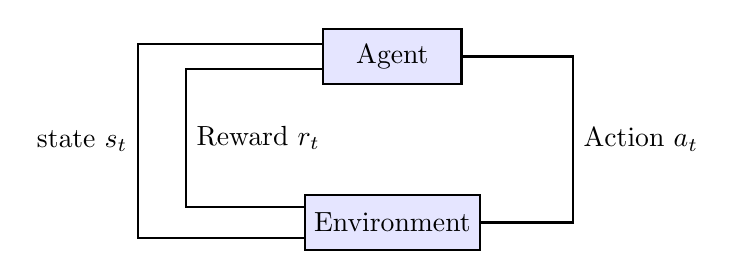
\begin{tikzpicture}[node distance = 6em, auto, thick]
		\node [block] (Agent) {Agent};
		\node [block, below of=Agent] (Environment) {Environment};
		
		\path [line] (Agent.0) --++ (4em,0em) |- node [near start]{Action $a_{t}$} (Environment.0);
		\path [line] (Environment.190) --++ (-6em,0em) |- node [near start] {state  $s_{t}$} (Agent.170);
		\path [line] (Environment.170) --++ (-4.25em,0em) |- node [near start, right] {Reward $r_{t}$} (Agent.190);
		\label{}
	\end{tikzpicture}
	\caption{Reinforcement learning schematic and the agent environment interaction.}
	\label{RL_agent}
\end{figure}

\begin{itemize}
	
	
	\item \textit{states} ($S_t \in \mathcal{S}$): A state (s) is a collection of all essential information about the current situation that can be used to forecast future states.  For example, in the case of a robot arm trying to grab a box, the current position of the robot arm could be the state. States can be a multidimensional discrete or continuous set. \\
	Sometimes, an observation of the states is available instead of the states themselves. For example, instead of a current position of the arm, a snapshot picture is available. 
	\item \textit{action} ($A_t \in \mathcal{A}$):   Actions are utilized to control the states by the agents \textit{policy}, which is a mapping from states to actions. It can be either stochastic $ a = \pi(.|s)$ or deterministic $a=\mu(s)$.  Actions somehow can be compared to the control input in the feedback of a control system. As an example, in a navigation problem, the actions are the torque applied to the wheels. Actions might belong to a discrete or continuous set, and they can also be multidimensional.
	\item \textit{Reward} ($R_t \in \mathcal{R} \subset \mathbb{R}$):  It is the measure of how well the agent is choosing the actions, to put it another way, how well is its \textit{policy}. For example, in the robot arm problem, it could be how close it is to grab the box.
	\item \textit{environment} $(p)$ : The environment is fully described by its \textit{dynamics} (distribution) which can be stochastic $s_{t+1} = p(.|s_t,a_t)$ or deterministic $s_{t+1} = p(s_t,a_t)$. Environment could be any sort of system in which a reward could be defined for a set of given actions applied to the environment. 	
	
\end{itemize}
The MDP framework is conceptual and adaptable, and it may be widely used in a variety of situations in several ways, including the stock price prediction \cite{lee2001stock} to low-level control of UAVs \cite{pi2020low}. Therefore, the definitions are different compared to a control platform. In an MDP, the interaction between the agent (controller) and the environment (the plant, controlled unit) happens in a discrete-time steps platform. The agent performs actions (control signal), receives the reward, and ends up being in a new state. Each interaction between the environment and the agent is called a \textit{step}. in each step the agent receives states $S_t$ and reward $R(s_t)$ from environment and generates a set of action(s) $A_t$  based on its policy which would transform the environment states to a new one $S_{t+1}$ based on transition probability $P(s_{t+1}|s_t,a_t)$ and consecutively provide with a $R_{t+1}$. So MDP can be defined as a tuple \cite{sutton2018reinforcement}:

\begin{equation}
	D\equiv (S, A, P, R)
\end{equation}
Expected Reward can be based on the current state and action $r = r(s,a)$:

\begin{equation}
	r(s,a) = \mathbb{E}[R_t|S_{t-1}=s,A_{t-1}]
\end{equation}
Or be based on the state-action-next state:

\begin{equation}
	r(s,a) = \mathbb{E}[R_t|S_{t-1}=s,A_{t-1},S_t=s']
\end{equation}
\subsubsection{Expected return}
Broadly speaking, the goal of a policy is to maximize the  average reward or discounted \textit{return} (a weighted average in which distant rewards have a less impact) in an episode\footnote{\textit{episode} consists of steps, starting from initial to terminal state, when the terminal state is reached, the process starts over from the initial state.}. In other words, the goal is to maximize the expected return $G_t$. There are different ways of defining the expected return \cite{kaelbling1996reinforcement}, here we discuss the one with discounted rate $\gamma \in (0,1)$ in an episode with T as final time step:\\

\begin{equation}
	G = R_{t}+\gamma R_{t+1}+ \gamma^2 R_{t+2}+ \dots + R_T\, \quad 0 \leq\gamma\leq 1 
\end{equation}

$\gamma$ is usually a number close to one since a low $\gamma$ can result in an instability \cite{kober2013reinforcement}. If $\gamma$ is chosen to be 1, then the approach is called average-reward criterion \cite{bertsekas2011dynamic}. In this case, it usually cannot distinguish between short-term transient reward, and it is mostly dominated by the steady-state region. If the policy achieves both acceptable short-term and long-term optimal behavior, then it is known as bias optimal \cite{lewis2002bias}. \\

\subsubsection{Value function}

The \textit{Value function} specifies how good a state is in an episode while a specific policy $\pi$ is followed. It can be based only on the state $V^\pi(s)$:
\begin{equation}
	\displaystyle V^\pi(s)= \mathbb{E}^{\pi}[G| s_t = s]
\end{equation}
where $\displaystyle \mathbb{E}_\pi$ denotes the expected return given that the agent follows policy. Note that the value of expected return should be calculated until terminal state is reached.
In a similar way the \textit{State-Action Value function} of acting $a$ in state (s) is defined as:
\begin{equation}
	\displaystyle Q^\pi(s,a)= \mathbb{E}^{\pi}[G|s_t=s,a_t=a]
\end{equation}

The value functions are policy dependent, meaning that the value of a state could be low in a policy while it would be high in another one; having this in mind, it is obvious that the optimal value functions are the ones obeying the optimal policy $\pi^*$:

\begin{equation}
	\displaystyle V^{\pi^*}(s)= \mathbb{E}^{\pi^*}[G| s_t = s]
\end{equation}

\begin{equation}
	\displaystyle Q^{\pi*}(s,a)= \mathbb{E}^{\pi^*}[G|s_t=s,a_t=a]
\end{equation}

$Q^{\pi*}(s,a)$ is the same as having the optimal policy because given the state (s) we can obtain the optimal policy from the below equation:

\begin{equation}
	a^*(s) =  \arg \max_a Q^*(s,a)
\end{equation}
\subsubsection{Bellman equation}
\textit{Bellman equation} expresses the value of a state, based on the value of its successor states. Bellman equation is obeyed in all the above equations for example in the Value function we have: 
\begin{equation}
	V^\pi(s_t) = R(s_t,\pi(s_t)) + \gamma \sum_{s_{t+1}} P(s_{t+1}|s_t,\pi(s_t)) V^\pi(s_{t+1}) 
\end{equation}

\begin{equation}
	V^{\pi^*}(s_t) = R(s_t,\pi^*(s_t)) + \gamma \sum_{s_{t+1}} P(s_{t+1}|s_t,\pi^*(s_t)) V^\pi(s_{t+1}) 
\end{equation}
In a situation with discrete actions, determining the optimal policy is simple, since an exhaustive search is possible if the optimal value function and the transition probabilities for the following states are known, however, in case of continuous spaces, function approximation methods are utilized.\\

There are numerous value function-based methods which has 3 major classes of:

\begin{enumerate}
	\item Dynamic programming-based methods.
	\item Monte Carlo methods
	\item Temporal difference methods.
\end{enumerate}

\subsection{Dynamic programming}

Dynamic Programming (DP) is well suited in a discrete scheme \cite{bucsoniu2010approximate}; however, it is possible to use it in a continuous framework. DP uses value functions to arrange and guide the search for optimal policies. The transition probability of the environment should be available, or it could be determined from experience.\\

In a DP algorithm \textit{policy iteration} is used, which is a process that alternates between \textit{policy evaluation} and \textit{policy improvement}. Initially, a random policy is used to start the approach, then the value function for the current policy is determined by policy evaluation. Each value of state in the current iteration is updated based on the values of the state in the previous iteration (bootstrapping), the policy $\pi$, and transition probability $p$. Finally, the policy is improved based on the most recent value function.

\subsection{Monte Carlo methods}

Unlike the DP, Monte Carlo methods learn directly from \textit{experience}\footnote{sampled episodes from environment} with no prior knowledge of MDP transitions. They carry out rollouts by executing the existing policy on the system, which is referred to as operating on-policy. The value function is updated after an episode is ended. This process is done using the average returns using the current experiences. The frequency of transitions and rewards is recorded and utilized to calculate value function estimates. As more episodes are produced, the average value will converge. The policy is improved by making it greedy regarding the value of the states. Although the method is quite simple, it is pretty powerful; for example, in the game of Tetris, this method outperforms most of the other ones \cite{gabillon2013approximate}.

\subsection{Temporal Difference}

Temporal Difference (TD) is a generalization of the Monte Carlo method. It also utilizes the bootstrapping of the DP so that TD(1) is the same as the Monte Carlo method, updating the values only when the episode is ended. TD(0) only considers the sampled successor states rather than the full distribution over the successor states in DP. In TD($\lambda$) ($0\geq\lambda\geq1$), values are updated before the end of the episode, and more than 1 step ahead is used.\\

Two popular TD approaches exist, with slightly different update procedures, state-action-reward-state-action (SARSA) \cite{rummery1994line}  and Q-learning \cite{watkins1992q}. SARSA uses the below equation for updating the Q value.

\begin{equation*}
	Q(s_t,a_t) \leftarrow Q(s_t,a_t) + \alpha [R_{t+1} + \gamma Q(x_{t+1},u_{t+1})-Q(s_t,u_t)]
\end{equation*}

While Q-learning uses:

\begin{equation}
	Q(s_t,a_t) \leftarrow Q(s_t,u_t) + \alpha [R_{t+1} + \gamma \max_{a_{t+1}} Q(x_{t+1},a_{t+1}) - Q(s_t,a_t)]
\end{equation}

SARSA is an on-policy algorithm, which means that its behavior and target policy are the same. Target policy is the output policy of the agent, which is used for evaluating the algorithm. The behavior policy $\pi_b$ is how the agent acts in exploration. Since exploratory policies are not optimal, \textit{on-policy} methods such as SARSA may quickly converge to a local optimum.\\

\textit{Off-policy} agents, such as Q-learning, employ different target and behavior policies; hence, they may use equal probability for taking actions in each state, so $\pi_b(a^*|s)>0$; as a result, they would find the optimal policy given enough time \cite{sutton1988learning}.\\

Value function methods struggle with the challenges of RL in robotic because they demand data to be filled into the entire state-action space, and they are intrinsically unstable \cite{szepesvari2010algorithms}. In addition, the bootstrapping will result in a bias if we want to use function approximation techniques which is inevitable in continuous spaces of robotics. As a result, value-based methods are not suitable for robotic applications, so we introduce a new family of RL methods called the policy search in the next section.

\section{Policy search}

Policy search approaches do not require using a value function model and instead search for the optimal policy. The concept behind this method is that it is feasible to enhance an episode's return without knowing the value of each state. The disadvantage of this technique is that it requires evaluating the policy and calculating the return in order to determine if the chosen policy is superior or not. Usually, a parameterized policy is chosen, and the parameters are tuned to maximize the expected return. This is usually done by methods such as gradient ascent \cite{baird1999reinforcement} or hill climbing \cite{kimura1995reinforcement}. \\

Policy searches provide many advantages. For example, it is feasible to take advantage of an expert for parameter initialization \cite{peters2006policy}, or it is possible to choose the suitable policy parameter structure, ensuring robustness and stability \cite{bertsekas2011dynamic}. Therefore, making policy search, a well-suited method for robotic which is proven by real system applications \cite{deisenroth2014multi, vikas2015model}.\\

In the case where gradient ascent is used for the optimization of the policy, we have: 
\begin{equation}
	J(\pi_{\kappa}) = \mathbb{E}^{\pi_{\kappa}}[G_{t}]
\end{equation}
\begin{equation}
	\kappa_{k+1}=\kappa_k+\alpha (\nabla_{\kappa} J(\pi_{\kappa})|_{\kappa=\kappa_k}
\end{equation}
In which, $\nabla_{\kappa} G_{\pi_{\kappa}}|$ is called \textit{policy gradient} \cite{sutton1999policy}. Which can be expressed as:

\begin{equation}
	\nabla_{\kappa} J_{\pi_{\kappa}} = \gamma^t G_{t}  \frac{\nabla_{\kappa} \pi_{\kappa}(a_t|s_t)}{\pi_{\kappa}(a_t|s_t)}
\end{equation}

\begin{equation}
	\nabla_{\kappa} J_{\pi_{\kappa}} = \gamma^t G_{t} \nabla_{\kappa}   \log \pi_{\kappa}(a_t|s_t) 
	\label{reinforce equation}
\end{equation}
The term $\nabla_{\kappa}   \log \pi_{\kappa}(a_t|s_t)$ is referred to as \textit{eligibility vector}.
Equation \ref{reinforce equation} is first introduced by \cite{williams1992simple} known as REINFORCE algorithm. This algorithm needs the episode to be terminated to calculate $G_t$, which is why this algorithm is considered a Monte Carlo algorithm. Methods such as Trusted Region Policy Optimization (TRPO) \cite{schulman2015trust} or Proximal Policy Optimization (PPO) \cite{schulman2017proximal} are examples of using such methodology.\\

For continuous actions, instead of learning the probability of the infinite number of actions, usually a Gaussian distribution is used:

\begin{equation}
	\pi(a|s,\kappa) = \frac{1}{a_\sigma(s,\kappa) \sqrt{2\pi}} exp\big( -\frac{(a-a_\mu(s,\kappa))^2}{2a_\sigma(s,\kappa)^2} \big)
\end{equation}

One of the methods to parameterize the policy is using a neural network named Deep Reinforcement Learning.

\subsection{Deep Reinforcement Learning}

In RL, neural networks (NN) are function approximation tools when the state or action space is continuous or too large. In some instances, it is simpler to approximate the value function, whereas, in others, it is easier to approximate policy. In latter cases, policy-based methods are more favorable as they yield a better asymptotic policy \cite{simsek2016most}. In both cases, a neural network can be employed for value approximation or policy approximation.\\

Neural networks can learn to map states to values or state-action pairs to Q values. Instead of using a lookup table to store, index, and update all possible states and their values - which is impossible with huge problems- We can train a neural network on samples from the state and action space to predict the value of states or which actions to take given a state.\\

Now that policy search is introduced, it is possible to discuss the next generation of RL, actor-critic methods.\\

\section{Actor-critic methods}

Actor-critic methods are policy search methods in which a bias is introduced through bootstrapping in order to improve learning speed and reduce variance. The actor-critic method to the REINFORCE is like the TD algorithm to the Monte Carlo methods. \\

If only one step of the return is considered, (like TD(0)) the general formula for an actor-critic method can be given as:
\begin{equation}
	\kappa_{k+1}=\kappa_k+\alpha \big(R_{t+1}+\gamma \hat{v}_\omega (S_{t+1})-\hat{v}_\omega(S_t)\big) \nabla_{\kappa}   \log \pi_{\kappa}(a_t|s_t)
\end{equation}

\section{Soft Actor Critic} \label{sacsection}

%DDPG, an algorithm that concurrently learns a deterministic policy and a Q-function by using each to improve the other, and SAC, a variant that uses stochastic policies, entropy regularization, and a few other tricks to stabilize learning and score higher than DDPG on standard benchmarks.
Soft Actor-Critic (SAC) is an actor-critic off-policy algorithm with a stochastic policy \cite{haarnoja2019soft,haarnoja2018soft}. It is inspired by stochastic policy optimization and Deep Deterministic Policy Gradient (DDPG) approaches \cite{lillicrap2015continuous}. It has similarities to Twin Delayed DDPG (TD3)  method \cite{fujimoto2018addressing} such that both use two clipped Q approximators. Since it is a stochastic method, it also benefits from something similar to target policy smoothing. Which makes it a potent tool in the robotic control field \cite{haarnoja2019learning}.\\


The main feature of the SAC algorithm is that it tries to balance a trade-off between expected return and entropy \cite{gray2011entropy}. The more the entropy, the higher the exploration, and the less the entropy, the higher the expected return in the short term. This is related to the exploration-exploitation trade-off: increasing entropy leads to more exploration, speeding up learning later. It can also prevent converging to futile local optimums.\\

Before we can discuss the further details of the algorithm, it is necessary to discuss the details of the usage of entropy in RL.
\subsection{Entropy-Regularized Reinforcement Learning}
The entropy-regularized reinforcement learning changes the goal of RL by including an entropy term, so that the optimal policy not only aims to increase the reward but also tries to increase its entropy at each visited state \cite{haarnoja2017reinforcement}. The temperature parameter $\alpha$ balance between exploration and exploitation in such way that by increasing $\alpha$ the policy would try to explore more by adding a stochastic term the reward importance. The formula for this method is:

\begin{equation}
	\pi^* = \arg \max_\pi \mathbb{E}_{\tau \sim \pi} [\sum_{t=0}^{T} \gamma^t \big( r(s_t,a_t,s_{t+1}) + \alpha H(\pi(.|s_t)) \big)]
\end{equation}

in which $H(\pi(.|s_t))$ is the entropy of a stochastic policy, given by:

\begin{equation}
	H(\pi(.|s_t)) =  \mathbb{E}[-\log \pi(.|s_t)]
\end{equation}

So, comparing a deterministic policy to an entropy regularized policy, when multiple actions are almost equally valuable, the policy commits equal probability mass to the actions instead of choosing the most valuable action. In this framework, the state value and the state-action value should be modified:

\begin{equation}
	V_\pi(s) = \mathbb{E}_{\tau \sim \pi}\Bigg[\sum_{t=0}^{T} \gamma^t \bigg( r\Big(s_t,a_t,s_{t+1}+\alpha H\big(\pi(.|s_t)\big)\Big) \bigg)|s_0=s\Bigg]
\end{equation}

\begin{equation}
	Q_\pi(s) =  \underset{\tau \sim \pi}{\mathbb{E}}\Bigg[\sum_{t=0}^{T} \gamma^t \bigg( r\Big(s_t,a_t,s_{t+1}+\alpha H\big(\pi(.|s_t)\big)\Big) \bigg)|s_0=s, a_0=a\Bigg]
\end{equation}

\subsection{SAC algorithm}

The SAC algorithm is given in Algorithm \ref{sac algorithm}. The Q functions are updated using the Mean Squared Bellman Error (MSBE)\\

\begin{equation}
	L(\delta_i, {\mathcal D}) = \underset{(s,a,r,s_{t+1},d) \sim {\mathcal D}}{{\mathbb{E}}}\left[
	\Bigg( Q_{\delta_i}(s,a) -  \underbrace{\big(r + \gamma \min Q_{\delta_{targ,j}}(s_{t+1}, a_{t+1}) - \alpha \log \pi_{\kappa}(a_{t+1}|s_{t+1})\big)}_{y(r,s_{t+1},d)} \Bigg)^2
	\right],
\end{equation}

In which D is the buffer of the algorithm in which the transitions are stored.
Hence the Q functions are updated by the following gradient:
\begin{align}
	& \delta_{i,new} = \delta_{i,old}+ l_{\delta} \nabla_{\delta_{i,old}} \frac{1}{|B|}\sum_{(s,a,r,s_{t+1},d) \in B} \left( Q_{\delta_{i,old}}(s,a) - y(r,s_{t+1},d) \right)^2 && \text{for } i=1,2
\end{align}
The policy is updated given:
\begin{equation}
	\max_{\kappa} \underset{s \sim \mathcal{D}, \xi \sim \mathcal{N}}{\mathbb{E}}{\min Q_{\delta_i}(s,a_{\kappa}(s,\xi)) - \alpha \log \pi_{\kappa}(a_{\kappa}(s,\xi)|s)},
\end{equation}
The policy is updated by:
\begin{equation}
	\kappa_{new}=\kappa_{old} + l_{\kappa}\nabla_{\kappa} \frac{1}{|\mathcal{B}|}\sum_{s \in \mathcal{B}} \Big(\min Q_{\delta_i}(s, a_{\kappa}(s)) - \alpha \log \pi_{\kappa} \left(\left. a_{\kappa}(s) \right| s\right) \Big)
\end{equation}
sampling $a_{\kappa}(s)$ from Gaussian distribution of policy $\pi_{\kappa}(\cdot|s)$ is done by the squashed Gaussian function:
\begin{equation}
	a_t = f_\kappa (s_t, \xi_t)
\end{equation}
\begin{equation}
	a_t = tanh(\mu_\kappa(s_t)+\sigma_\kappa(s_t) \cdot \xi_t), \quad \quad \xi \in \mathcal{N} (0,I)
\end{equation}
However, after convergence is reached in order to evaluate the policy, the randomness term of the action is omitted to improve performance:
\begin{equation}
	\bar{a}_t = tanh(\mu_\kappa(s_t))
\end{equation}

\newpage
\begin{algorithm}[H]
	\caption{Soft Actor-Critic}
	\label{alg1}
	\begin{algorithmic}[1]
		\STATE \textbf{Initialization}: initialize policy parameters $\theta$
		\STATE initialize Q-function parameters $\delta_1$, $\delta_2$
		\STATE initialize target network parameters $\delta_{\text{targ},1} \leftarrow \delta_1$, $\delta_{\text{targ},2} \leftarrow \delta_2$
		\STATE initializing the replay pool $\mathcal{D}$
		\REPEAT
		\REPEAT
		\STATE  sample action $a \sim \pi_{\theta}(\cdot|s)$ 
		\STATE observe next state $s_{t+1}$ reward $r$ and done signal $d  \in [\text{TRUE},\text{FALSE}]$
		\STATE save $(s_t,a_t,r(s_t,a_t),s_{t+1},d)$ in replay pool $\mathcal{D}$
		\IF  {d is \textbf{TRUE}}
		\STATE reset environment state.
		\ENDIF
		\UNTIL{ $\mathcal{D}>\mathcal{D}_{min}$}
		\STATE  sample action $a \sim \pi_{\theta}(\cdot|s)$ 
		\STATE observe next state $s_{t+1}$ reward $r$ and done signal $d  \in [\text{TRUE},\text{FALSE}]$
		\STATE save $(s_t,a_t,r(s_t,a_t),s_{t+1},d)$ in replay pool $\mathcal{D}$
		\IF  {d is \textbf{TRUE}}
		\STATE reset environment state.
		\ENDIF
		\IF{it's time to update the parameters}
		\FOR{$j$ in range(however many updates)}
		\STATE sample a batch of transitions, $\mathcal{B} = \{ (s,a,r,s_{t+1},d) \}$ from $\mathcal{D}$
		\STATE Update Q-functions.
		\STATE Update policy.
		\STATE Update target networks by linearization 
		\begin{align*}
			\delta_{\text{targ},i} &\leftarrow \eta \delta_{\text{targ}, i} + (1-\eta) \delta_i && \text{for } i=1,2 \\
		\kappa_{\text{targ}}&\leftarrow \eta \kappa_{\text{targ}} + (1-\eta) \kappa
		\end{align*}
		\ENDFOR
		\ENDIF
		\STATE evaluate the policy to check the convergence using $\bar{a}_t$
		\UNTIL {convergence}
		\STATE \textbf{Return} $\kappa, \delta_1$ and $\delta_2$
	\end{algorithmic}
	\caption{sac algorithm}
	\label{sac algorithm}
\end{algorithm}

\chapter{Simulation Environment}
\section{Introduction}
Small-scale helicopters are highly nonlinear systems with complex coupling. Analyzing velocity fields around the rotor requires complicated experiments and numerical methods, which differ in each flight regime such as hover, stall, etc. \cite{doerffer2008numerical,crittenden2004combustion,patterson1990computational}. There are numerous studies on mathematical models of the helicopter dynamics and governing equations of the forces and moments applied to it \cite{padfield2008helicopter,marques2017advanced, seddon2011basic}. For this study, we have used the model already developed for the Evolution-EX helicopter in \cite{pourrezaei2014control}. Here we briefly discuss the model development of this helicopter.
\section{Governing equations}
A combination of four subsystems describes the Evolution-EX helicopter's (EEH) dynamics: the rigid-body dynamics of the fuselage, the main rotor, the tail rotor, and the empennage. Two frameworks are defined like other dynamic problems: the body (B) and the Inertia (I)  framework. 
\subsection{States and control input}
The states regarding the UAV dynamics include the velocity vector $[3\times1]$:

\begin{equation}
	V=[u,v,w]^T	
\end{equation}

In this equation, u denotes the velocity in the x direction, v represents the velocity in the y direction, and w is the velocity in the z direction.
and the angular velocity vector $[3\times1]$:

\begin{equation}
	\omega=[p,q,r]^T
\end{equation}

In this equation, p represents represent the angular velocity in the p direction, q denotes the angular velocity in the y direction, and r is the angular velocity in the z direction.
with respect to body coordinates {B} and the position vector $[3\times1]$:

\begin{equation}
	p=[x,y,z]^T
\end{equation}

and the Euler angles vector which is roll pitch and yaw $[3\times1]$:

\begin{equation}
	\Theta=[\phi,\theta,\psi]^T
\end{equation}

with respect to inertia framework {I} and the input vector $[4\times1]$:

\begin{equation}
	U=[\delta_{col},\delta_{lat},\delta_{lon},\delta_{ped}]^T
\end{equation} 

the $\delta_{col}$ is the collective input which is responsible for increasing the angle of attack in all the angles of the blade plane, the lateral input $\delta_{lat}$ is responsible to increase the angle of attack for a lateral movement of the helicopter and $\delta_{lon}$ on the other hand is doing the same thing for a longitudinal movement. The $\delta_{ped}$ increases the angle of attack of the blades for the tail rotor in the same way that $\delta_{col}$ does for the main rotor blades.
In the next section the governing equations regarding the states are discussed

\subsection{State-space equations}

The Newton-Euler equations of motion of the helicopter fuselage are defined as:

\begin{equation}\label{eq1}
	\dot{V}=\frac{1}{m} F-\omega\times V
\end{equation}

\begin{equation}\label{eq2}
	\dot{\omega}=I^{-1}M-I^{-1}(\omega \times I \omega) 
\end{equation}

\begin{equation}
	\dot{\Theta}=\Phi(\Theta)\omega 
\end{equation}

\begin{equation}
	\dot{p}=R_{b}^I(\Theta)V
\end{equation}

F and M are defined as vector of external forces and moments respectively. Derivation of F and M are elaborated in \ref{force section} and \ref{Moment section} respectively. $R_b^I$ and $\Phi$ are linear and angular velocity transformation matrices given as follows: 
\begin{gather}
	R_b^I
	=
	\begin{bmatrix}
		s(\theta)c(\psi) &
		-c(\phi)sin(\psi)+s(\phi)s(\theta)c(\psi)&
		s(\phi)s(\psi)+c(\phi)s(\theta)c(\psi) \\
		c(\theta)s(\psi) &
		c(\phi)c(\psi)+s(\phi)s(\theta)s(\psi)&
		-s(\phi)c(\psi)+c(\phi)s(\theta)s(\psi)\\
		-s(\theta)&
		s(\phi)c(\theta)&
		c(\phi)c(\theta)
	\end{bmatrix}
\end{gather}

\begin{gather}
	\Phi
	=
	\begin{bmatrix}
		1 &
		s(\phi)t(\theta)&
		c(\phi)t(\theta) \\
		0 &
		c(\phi)&
		-s(\phi)\\
		0&
		\frac{s(\phi)}{c(\theta)} &
		\frac{c(\phi)}{c(\theta)}
	\end{bmatrix}
\end{gather}

in which s, c and t stands for "sin", "cos" and "tan" respectively.
The I is the moment of inertia in which the off-diagonal terms are neglected:

\begin{equation}
	I=
	\begin{bmatrix}
		I_{xx} &
		0&
		0 \\
		0 &
		I_{yy}&
		0\\
		0&
		0&
		I_{zz}
	\end{bmatrix}
\end{equation}

The $I_{xx}$, $I_{yy}$ and $I_{zz}$ are the rolling, pitching and yawning moment of inertia.\\

In the following sections, equations regarding the derivation of forces and moments in \ref{eq1} and \ref{eq2} are introduced.
\subsection{Blade flapping}

The dynamics of main rotor and stabilizer bar of the EEH is modeled by \textit{hybrid model approach} \cite{mettler2002system}. In this approach $\dot{a}$ and $\dot{b}$ are  tip-path-plane (TPP) longitudinal and lateral flapping angles respectively and the coefficients of first harmonic approximation in the Fourier series form. The rotor flapping state equations are:

\begin{equation}
	\dot{a}=-q-\frac{a}{\tau_{f}}+\frac{1}{\tau_{f}}(K_u\mu_x+K_w\mu_z)+\frac{A_{lon}}{\tau_{f}} (\delta_{lon}+K_c c)+A_b\frac{b}{\tau_{f}}
\end{equation}

\begin{equation}
	\dot{b} = -p-\frac{b}{\tau_{f}}+\frac{1}{\tau_{f}}(K_v\mu_y)+\frac{B_{lat}}{\tau_{f}}(\delta_{lat}+K_d d)+B_a \frac{a}{\tau_{f}}
\end{equation}

$K_u$ is the flapping due to the forward velocity factor, the $K_v$ on the other hands denotes the flapping due to the side-way velocity factor. In the same way, $K_w$ is considered to be te flapping due to downward velocity factor. $K_c$ reflects the longitudinal flapping due to the stabilizer bar factor and $K_d$ depicts the lateral flapping due to the stabilizer bar factor. $A_{lon}$ denotes the longitudinal cyclic to flap gain at nominal rpm and $B_{lat}$ is the lateral cyclic to flap gain at nominal rpm. Last but not least, the $\tau_f$ is the main rotor flapping time-constant.\\
$\mu_x,\mu_y$ and $\mu_z $ are the non-dimensional airflow components defined as:

\begin{equation}
	\begin{aligned}
		\mu_x&=\frac{u-u_{wind}}{\Omega R_{mr}}\\
		\mu_y&=\frac{v-v_{wind}}{\Omega R_{mr}} \\
		\mu_z&= \frac{w-w_{wind}}{\Omega R_{mr}}\\
	\end{aligned}
\end{equation}

And the $K_{u}$, $K_v$ and $K_w$ are given by:

\begin{equation}
	K_{u}=2K_{\mu}(\frac{4}{3}\delta_{col}-\frac{Vi}{\omega R_{mr}})
\end{equation}

\begin{equation}
	K_v=-K_u
\end{equation}

\begin{equation}
	K_w=16K_{\mu} \mu_{mr}^2 \frac{sign(\mu_{mr})}{(1-\mu_{mr}^2/2)*(8sign(\mu_{mr})+CL_\alpha \sigma)}
\end{equation}

The stabilizer bar state equations c and d are TPP longitudinal and lateral flapping angles of the stabilizer bar given by:

\begin{equation}
	\dot{c}=-q-\frac{c}{\tau_s}+\frac{C_{lon}}{\tau_s}\delta_{lon}
\end{equation}

\begin{equation}
	\dot{d}=-p-\frac{d}{\tau_s}+\frac{D_{lat}}{\tau_s}\delta_{lat}
\end{equation} 

\subsection{Force derivation} \label{force section}
 \tikzset{
	every label/.append style={font=\scriptsize},
	my edge labels/.style={font=\scriptsize},
	dominant/.append style={label=below:$dominant$},
}


The force is derived as follows:

\begin{equation}
	F= 
	\begin{bmatrix}
		F_x \\
		F_y\\
		F_z\\
	\end{bmatrix}
	+R_b^I \begin{bmatrix}
		0 \\
		0\\
		mg\\
	\end{bmatrix}
\end{equation}

in which $F_x$, $F_y$ and $F_z$ are defined as:

\begin{equation}
	F_x=-a\ T_{mr}+F_{x,fus}
\end{equation}

\begin{equation}
	F_y=b\ T_{mr}+T_{tr}+F_{y,fus} + F_{y,vt}
\end{equation}

\begin{equation}
	F_z=-T_{mr}+F_{z,fus} + F_{z,ht}
\end{equation}

$T_{mr}$ is the main rotor thrust and $T_{tr}$ denotes the tail rotor thrust. $T_{mr}$ is given by:

\begin{equation}
	T_{mr} = \textbf{f}_{T_{mr}}+\textbf{b}_{T_{mr}}U;
	\label{T_mr}
\end{equation}

in which $\textbf{f}_{T_{mr}}$ is the autonomous term of the main rotor thrust:

\begin{equation}\label{f_t}
	\textbf{f}_{T_{mr}}= \frac{1}{4} \rho \pi R_{mr}^4\Omega^2\sigma_{mr}(C_{L_{0}}(\frac{2}{3}+\mu_x^2+\mu_y^2)+C_{L_{\alpha}}(\mu_z-\lambda_0))
\end{equation}

In which $R_{mr}$ is the main rotor radius and $\Omega$ represents the nominal main rotor speed. $\sigma_{mr}$ depicts the main rotor solidity factor and $C_{L0}$ and $C_{L\alpha}$ are the main rotor blade zero lift curve and blade lift curve slope respectively.\\
$\lambda_0$ is the inflow ratio expressed as:

\begin{equation}
	\lambda_0=\frac{V_i}{\Omega R_{mr}}
\end{equation}

The solidity factor derived by:

\begin{equation}
	\sigma_{mr}=\frac{Nc_{mr}}{\pi R_{mr}}
\end{equation}

and $b_{T_{mr}}$ in \ref{T_mr} is control input coefficient term given by:

\begin{equation}\label{b_T}
	\textbf{b}_{T_{mr}}= \frac{1}{4} \rho \pi R_{mr}^4 \Omega^2 \sigma_{mr} C_{L_{\alpha}}\begin{bmatrix}
		\mu_x^2+\mu_y^2+\frac{2}{3}&
		-\mu_y&
		\mu_x&
		0
	\end{bmatrix}
\end{equation}

Similarly, it is possible to derive the tail rotor thrust $T_{tr}$:

\begin{equation}
	T_{tr} = \textbf{f}_{T_{tr}}+\textbf{b}_{T_{tr}}U;
\end{equation}

In which $\textbf{f}_{T_{tr}}$ is the autonomous term of the tail rotor thrust:

\begin{equation}\label{f_t_tr}
	\textbf{f}_{T_{tr}}=- \frac{1}{4} \rho \pi R_{tr}^4 n_{tr}^2\Omega^2\sigma_{tr}C_{L\alpha_{tr}}v_{tail}
\end{equation}

And input coefficients $b_{T_{tr}}$ is given by:

\begin{equation}\label{b_Ttr}
	\textbf{b}_{T_{tr}}= -\frac{1}{4} \rho \pi R_{tr}^4 n_{tr}^2 \Omega^2 \sigma_{tr} C_{L\alpha_{tr}}\begin{bmatrix}
		0&
		0&
		0&
		u_{tail}^2+w_{tail}^2+\frac{2}{3}
	\end{bmatrix}
\end{equation}

The normalized velocities at tail rotor can be given as:

\begin{equation}
	\begin{aligned}
		u_{tail}&=\frac{u-u_{wind}}{\Omega_{tr} R_{tr} }\\
		v_{tail}&=\frac{v-v_{wind}-V_{i_{tr}}+x_{fus}r}{\Omega_{tr} R_{tr}} \\
		w_{tail}&= \frac{w-w_{wind}-K_{\lambda}V_i+x_{fus}q}{\Omega_{tr} R_{tr}}\\
	\end{aligned}
\end{equation}

The tail rotor nominal speed is given by:

\begin{equation}
			\Omega_{tr}=n_{tr}\Omega  
\end{equation}

In which the $n_{tr}$ is gear ratio of tail rotor to main rotor. $F_{y,vt}$ is the vertical tail force derived by:

\begin{equation}\label{Yvt}
	F_{y,vt}=\frac{1}{2} \rho S_{vt} \Big( C_{L_\alpha}^{vt}V_{vt}(v-v_{wind})+v_{tail}^2 \Big)
\end{equation}

In the above equation, the $\rho$ is the air density. $S_{vt}$ denotes the vertical tail area, 
And horizontal tail force $F_{z,ht}$ is:

\begin{equation} \label{Z_ht}
	F_{z,ht}=\frac{1}{2} S_{ht} \Big( C_{L_{\alpha}}^{ht} \mid u-u_{wind} \mid w_{ht} +w_{ht}^2 \Big)    
\end{equation}

In equation \ref{Yvt} $V_{vt}$ and $v_{tail}$ are axial and normal velocities in vertical tale defined as:

\begin{equation}
	\begin{aligned}
		V_{vt}&=\sqrt{(u-u_{wind})^2+(w- w_{wind} +x_{vt}q-K_\lambda V_i)^2}\\
		v_{tail}&=v-v_{wind}+x_{vt}r-V_{i_{tr}} \\
	\end{aligned}
\end{equation}

Similarly in equation $w_{ht}$ is the horizontal tail velocity in the z direction \ref{Z_ht}:

\begin{equation}
	w_{ht}=w-w_{wind}-x_{ht}q-K_{\lambda}V_i
\end{equation} 

The $K_{\lambda}$ is the main rotor downwash factor at fuselage.\\

$F_{z,fus} , F_{y,fus}$ and $F_{x,fus}$ are drag forces derived by:

\begin{equation}
	F_{x,fus}=-\frac{1}{2} \rho S_x^{fus} V_{fus} (u-u_{wind})
	\label{X_fus}
\end{equation}

\begin{equation}\label{Y_fus}
	F_{y,fus}=-\frac{1}{2} \rho S_y^{fus} V_{fus} (v-v_{wind})
\end{equation}

\begin{equation}\label{Z_fus}
	F_{z,fus}=-\frac{1}{2} \rho S_z^{fus} V_{fus} (w-w_{wind}+V_i)
\end{equation}

the dynamic pressure of the fuselage $V_{fus}$ in expression \ref{X_fus} is defined as:

\begin{equation}
	V_{fus}=\sqrt{(u-u_{wind})^2+(v-v_{wind})^2+(w-w_{wind}+V_i)^2}
\end{equation}

\subsection{Moment derivation} \label{Moment section}

Moment includes 3 terms roll, pitch and yaw:

\begin{equation}
	M =\begin{bmatrix}
		M_{roll}\\
		M_{pitch}\\
		M_{yaw}\\
	\end{bmatrix}
\end{equation}

The three terms in the above equation are given as:

\begin{equation}
	M_{roll} = (K_{\beta}-T_{mr}Z_{cg})b;%-Ttail*z_fus;
\end{equation}

\begin{equation}
	M_{pitch} = (K_\beta-T_{mr}Z_{cg})a;
\end{equation}

\begin{equation}
	M_{yaw} = Q_{mr}+T_{tr}x_{fus};
\end{equation}

$Z_{cg}$ is the Main rotor hub height from center of gravity and $x_{fus}$ is the tail rotor hub offset from center of gravity along x-axis.
Main rotor drag torque $Q_{mr}$ is derived by:
\begin{equation}
	Q_{mr} = \textbf{f}_{Q_{mr}}+\textbf{b}_{Q_{mr}}U;
\end{equation}
In which the main rotor drag torque terms are given as:
\begin{equation} \label{f_Q}
	\textbf{f}_{Q_{mr}}=\frac{1}{8} \rho \pi R_{mr}^5 \Omega^2 \sigma_{mr} C_{L_{\alpha}}  \bigg( \frac{C_{D0}}{C_{L_{\alpha}}} \Big( \mu_x^2+\mu_y^2+1 \Big)-2(\mu_{z}-\lambda_0)^2 \bigg)
\end{equation}
\begin{equation} \label{b_Q}
	\textbf{b}_{Q_{mr}}=\frac{1}{8} \rho \pi R_{mr}^5 \Omega^2 \sigma_{mr} C_{L_{\alpha}} (\lambda_0-\mu_z)  \begin{bmatrix}
		\frac{4}{3}
		-\mu_y&
		\mu_x &
		0
	\end{bmatrix}  
\end{equation}

\subsection{Induced velocity}

As indicated in \cite{johnson2012helicopter} and \cite{leishman2006principles} the blade element analysis considers each blade
element as a two-dimensional airfoil. The aerodynamic behavior of neighboring
blade elements is independent of each other. An induced inflow velocity on each
blade element should be accounted for, which is a product of the rotor wake. Analytical
ways of calculating the induced velocity may be found using momentum theory,
vortex theory, or nonuniform inflow calculations \cite{johnson2012helicopter}.\\

In general, the inflow velocity calculation is a challenging task due to its non-uniformity across the blade span; mathematical simplifications should be applied to minimize the complexity of the analysis. Finally, after determining the velocity components
of the blade element, the aerodynamic forces acting on this element are calculated.
The complete dynamic behavior of the blade is obtained by integrating the applied
forces of the individual elements throughout the blade span. Here we use an experimental approach for induced velocity. \\

$V_i$ and $V_{i_{tr}}$ are induced velocity in main rotor and tail rotor respectively. $V_i$ is given by:

\begin{equation}
	V_i=\frac{v_a}{\sqrt{1+\bar{\mu}^2}}
\end{equation}

In which:

\begin{equation}
	V_h=\sqrt{mg/(2\rho \pi R_{mr}^2)}
\end{equation}

\begin{equation}
	\mu=\sqrt{\mu_x^2+\mu_y^2} 
\end{equation}

\begin{equation}
	\bar{\mu}=\frac{\mu}{V_h/(\Omega R_{mr})} 
\end{equation}

\begin{equation}
	V_a=-\frac{w-w_{wind}}{V_h}
\end{equation}

\begin{equation}
	v_a = \left\{
	\begin{array}{ll}
		-\frac{1}{2} V_a-\sqrt{\frac{V_a^2}{4}-1} & \mbox{if } \ V_a 	\leqslant -2 \\
		1-\frac{1}{2} V_a+\frac{25}{12} V_a^2 +\frac{7}{6} V_a^3 & \mbox{if } \ -2<V_a<0 \\
		-\frac{1}{2} V_a+\sqrt{\frac{V_a^2}{4}+1} & \mbox{if } \ V_a	\geqslant 0 \\
	\end{array}
	\right.
	\label{vamr}
\end{equation}

Similarly, $V_{i_{tr}}$ is:

\begin{equation}
	V_{i_{tr}}=\frac{v_{a_{tr}}}{\sqrt{1+\overline{\mu_{tr}}^2}}
\end{equation}

In which:

\begin{equation}
	V_{h_{tr}}=\sqrt{f_{F_{y,mr}}/(2\rho \pi R_{tr}^2 x_{fus} )}
\end{equation}

\begin{equation}
	\mu_{tr}=\sqrt{u_{tail}^2+w_{tail}^2} 
\end{equation}

The $\overline{\mu}_{tr}$ is the advance ratio normalized by $V_{h_{tr}}/(\Omega R_{tr}$:

\begin{equation}
	\overline{\mu}_{tr}=\frac{\mu_{tr}}{V_{h_{tr}}/(\Omega R_{tr})} 
\end{equation}

\begin{equation}
	V_{a_{tr}}=-\frac{v-v_{wind}+x_{fus}r}{V_h}
\end{equation}

\begin{equation}
	v_{a_{tr}} = \left\{
	\begin{array}{ll}
		-\frac{1}{2} V_{a_{tr}}-\sqrt{\frac{V_{a_{tr}}^2}{4}-1} & \mbox{if } \ V_{a_{tr}} 	\leqslant -2 \\
		1-\frac{1}{2} V_{a_{tr}}+\frac{25}{12} V_{a_{tr}}^2 +\frac{7}{6} V_{a_{tr}}^3 & \mbox{if } \ -2<V_{a_{tr}}<0 \\
		-\frac{1}{2} V_{a_{tr}}+\sqrt{\frac{V_{a_{tr}}^2}{4}+1} & \mbox{if } \ V_{a_{tr}}	\geqslant 0 \\
	\end{array}
	\right.
	\label{vatr}
\end{equation}

Instead of using equation \ref{vamr} and \ref{vatr}, we use the following approximate functions by regression as they provide a faster calculation time in simulations:

\begin{equation}
	v'_a = \frac{4.055}{{\left(1.28V_{a}+1.45\right)}^2+1.7}+0.066
\end{equation}

\begin{equation}
	v'_{a_{tr}} = \frac{4.055}{{\left(1.28V_{a_{tr}}+1.45\right)}^2+1.7}+0.066
\end{equation}

Figure \ref{fig_va} depicts the two functions $v_a$ and $v'_a$ based on $V_a$.

\begin{figure}
	\begin{center}
		{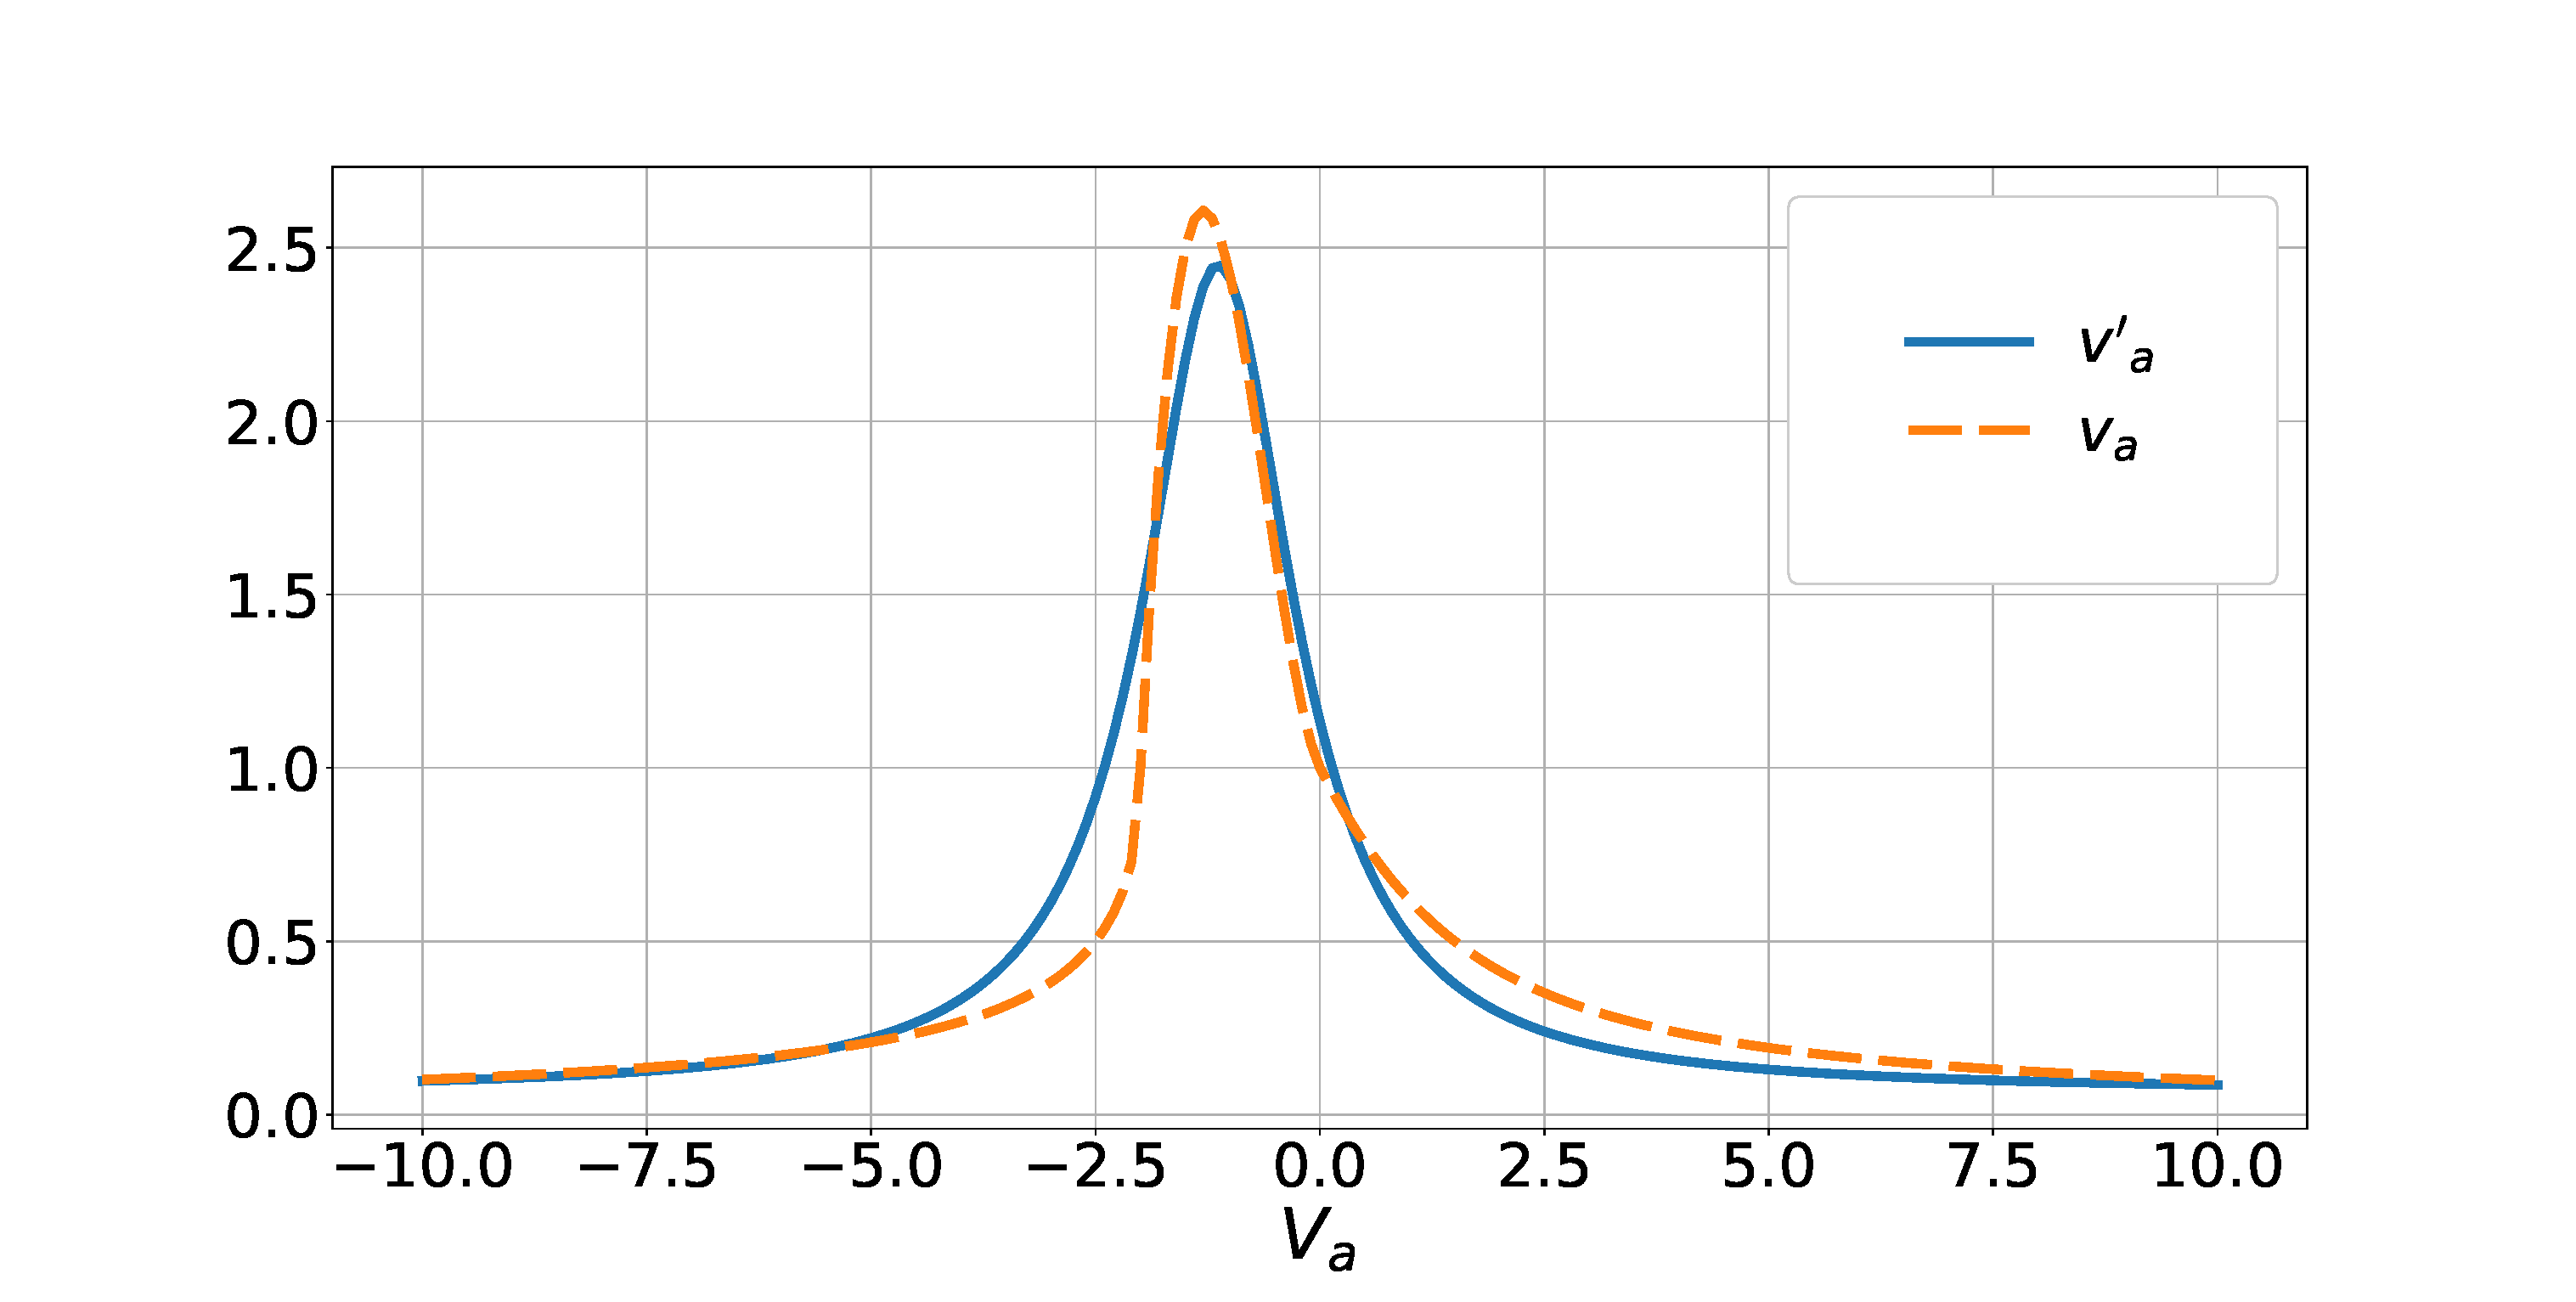
\includegraphics[scale=0.3]{va.eps}}
		
		\caption{Function approximation of $v_a$ by $v'_a$, $R^2=0.947$.}
		\label{fig_va}
	\end{center}
\end{figure}

The constant parameters in the above modeling is given in the table \ref{helicopter_parameters}.
\begin{longtable}{c|c|c||c|c|c} 
	\caption {Constant parameters in the helicopter modeling}\label{helicopter_parameters}\\\toprule
	\endfirsthead
	\caption* {\textbf{Table \ref{helicopter_parameters} Continued:} }\\\toprule
	\endhead
	\endfoot
	\bottomrule
	\endlastfoot
	\textbf{Parameter} & \textbf{Value} & \textbf{Dimension} & \textbf{Parameter} & \textbf{Value} & \textbf{Dimension} \\ \hline \hline
	$\alpha_{1}$ & $53$ &  $[-]$ & $\alpha_{2}$ & $55$ &  $[-]$ \\  \hline
	$ \Omega$ & $115 $ &  $[rad/s]$ & $\rho $ & $1.107 $ &  $[kg/m^3]$ \\ \hline
	$ \tau_f$ & $0.04 $ &  $[s]$ & $\tau_s $ & $ 0.2$ &  $[s]$ \\ \hline
	$\tau_s $ & $ 0.2$ &  $[s]$ & $A_b $ & $-0.1 $ &  $ [-]$ \\ \hline
	$A_{lon} $ & $ 1$ &  $[-]$ & $B_a $ & $0.1 $ &  $ [-]$ \\ \hline
	$B_{lat} $ & $0.9875 $ &  $[-]$ &$C_{D0_{tr}} $ & $0.06 $ &  $[-]$  \\ \hline
	$C_{D0} $ & $0.01 $ &  $[-]$ & $C_{L0} $ & $0.008 $ &  $[-]$ \\ \hline
	$C_{L\alpha_{tr}} $ & $4.95 $ &  $[rad^{-1}]$ & $C_{L\alpha} $ & $5.49 $ &  $[rad^{-1}]$ \\ \hline
	$c_{mr} $ & $0.082 $ &  $[m]$ & $c_{tr} $ & $0.025 $ &  $[m]$ \\ \hline
	$I_{xx} $ & $ 0.3$ &  $[kg.m^2] $  & $I_{yy}$ & $1.6$ & $[kg.m^2]$ \\ \hline
	$I_{zz} $ & $2.0 $ &  $[kg.m^2]$ & $K_\lambda $ & $1 $ &  $[-] $ \\ \hline
	$K_s $ & $0.3 $ &  $[-] $  & $K_\beta $ & $ 255$ &  $[N.m]$ \\ \hline
	$K_{lat} $ & $0.98 $ &  $[-] $  & $K_{lon} $ & $1 $ &  $[-] $ \\ \hline
	$m $ & $11.5 $ &  $[kg] $  & $n_{tr} $ & $6 $ &  $[-] $ \\ \hline
	$R_{mr} $ & $0.95 $ &  $[m]$  & $R_{tr} $ & $0.15 $ &  $[m] $ \\ \hline
	$S_x^{fus} $ & $0.1 $ &  $[m^2] $  & $S_y^{fus} $ & $0.83 $ &  $[m^2] $ \\ \hline
	$S_z^{fus} $ & $0.51 $ &  $[m^2] $  & $x_{fus} $ & $-1.22 $ &  $[m] $ \\ \hline
	$z_{CG}$ & $-0.32 $ &  $[m] $  &  &  & \\ 
\end{longtable}

\section{Sliding mode control}
In order to compare the results obtained by the RL method to a traditional control method, we here provide the details of a sliding mode controller as a nonlinear method. As it is an under actuated system which means that there are only have 4 inputs and 6 states to control. Based on \cite{slotine1991applied,pourrezaei2014control} in order to use sliding mode controller on a helicopter, first we have to change it to a square and affine in control form  so  we discuss how this is achieved.

\subsection{Force derivation in control affine form} \label{force section_affine}
In order to provide a control input by sliding mode controller, each of the force and moment should be linearized based on the control input. Control-affine form of each term is given as a input coefficient "b" and a "f" term which is related to autonomous response of the system. Force is given as:

\begin{equation}\label{Force eq}
	F=\textbf{f}_F+\textbf{b}_FU
\end{equation}

$f_F$ is the autonomous term of the force expressed as:
\begin{gather}\label{F_0}
	\textbf{f}_F
	=
	\begin{bmatrix}
		\textbf{f}_{F_{x,mr}}+F_{x,fus} \\
		\textbf{f}_{F_{y,mr}}+\textbf{f}_{F_{y,tr}}+F_{y,vt}+F_{y,fus}\\
		\textbf{f}_{F_{z,mr}}+F_{z,ht}+F_{z,fus} \\
	\end{bmatrix}
	+R_b^{I^{-1}}\begin{bmatrix}
		0 \\
		0\\
		mg \\
	\end{bmatrix}
\end{gather}

in which:

\begin{equation}\label{f_X_MR}
	\textbf{f}_{F_{x,mr}}=\textbf{f}_T(\tau_f q-a_v)
\end{equation}
 
\begin{equation}
	F_{x,fus}=-\frac{1}{2} \rho S_x^{fus} V_{fus} (u-u_{wind})
	\label{X_fus}
\end{equation}

\begin{gather}\label{f_Y_MR}
	\textbf{f}_{F_{y,mr}}=(\tau_fp+b_v)\textbf{f}_T
\end{gather}

\begin{equation}
	\textbf{f}_{F_{y,tr}}=\textbf{f}_{T_{tr}} 
\end{equation}



\begin{equation}
	\textbf{f}_{F_{z,mr}}=-\textbf{f}_T    
\end{equation}


$a_v$ and $b_v$ in \ref{f_X_MR} and \ref{f_Y_MR} are respectively longitudinal and lateral translational velocity contributions to the flapping of the main rotor  and defined by the following terms:

\begin{equation}
	\begin{aligned}
		a_v&=\frac{\partial a_1}{\partial \mu_x} \mu_x+\frac{\partial a_1}{\partial \mu_z} \mu_z \\
		b_v&=\frac{\partial a_1}{\partial \mu_y}\mu_y 
	\end{aligned}
\end{equation}

the dynamic pressure of the fuselage in expression \ref{X_fus} is defined as:

\begin{equation}
	V_{fus}=\sqrt{(u-u_{wind})^2+(v-v_{wind})^2+(w-w_{wind}+V_i)^2}
\end{equation}



$\textbf{f}_{T_{mr}}$ is the main rotor thrust autonomous term in the control affine form given by \ref{f_t}.
and $\lambda_0$ is the inflow ratio expressed as:

\begin{equation}
	\lambda_0=\frac{V_i}{\Omega R_{mr}}
\end{equation}

$\sigma_{mr}$ is the solidity factor derived by:

\begin{equation}
	\sigma_{mr}=\frac{Nc_{mr}}{\pi R_{mr}}
\end{equation}

The velocities at tail rotor can be normalized given as:

\begin{equation}
	\begin{aligned}
		u_{tail}&=\frac{u-u_{wind}}{\Omega_{tr} R_{tr} }\\
		v_{tail}&=\frac{v-v_{wind}-V_{i_{tr}}+x_{fus}r}{\Omega_{tr} R_{tr}} \\
		w_{tail}&= \frac{w-w_{wind}-K_{\lambda}V_i+x_{fus}q}{\Omega_{tr} R_{tr}}\\
		\Omega_{tr}&=n_{tr}\Omega  
	\end{aligned}
\end{equation}

similarly velocities at vertical tail or horizontal tail can be defined.\\ 
In equation \ref{Yvt} $V_vt$ and $v_{tail}$ are axial and normal velocities in vertical tale defined as:

\begin{equation}
	\begin{aligned}
		V_{vt}&=\sqrt{(u-u_{wind})^2+(w- w_{wind} +x_{vt}q-K_\lambda V_i)^2}\\
		v_{tail}&=v-v_{wind}+x_{vt}r-V_{i_{tr}} \\
	\end{aligned}
\end{equation}

Similarly in equation \ref{Z_ht}:

\begin{equation}
	w_{ht}=w-w_{wind}-x_{ht}q-K_{\lambda}V_i
\end{equation} 

$b_F$ in equation \ref{Force eq} is the input coefficient of the force which is defined as:

\begin{gather}\label{F_U}
	\textbf{b}_F
	=
	\begin{bmatrix}
		\textbf{b}_{F_{x,mr}}\\
		\textbf{b}_{F_{y,mr}}+\textbf{b}_{F_{y,tr}}\\
		\textbf{b}_{F_{z,mr}}\\
	\end{bmatrix}
\end{gather}

In which the following terms are used:

\begin{equation}
	\textbf{b}_{F_{x,mr}}=(\tau_f q-a_v)\textbf{b}_T-\begin{bmatrix}
		0&0&K_{lon}\textbf{f}_T&0
	\end{bmatrix}
\end{equation}

\begin{gather}
	\textbf{b}_{F_{y,mr}}=(-\tau_fp+b_v)\textbf{b}_T- \begin{bmatrix}
		0&K_{lat}\textbf{f}_T&0&0
	\end{bmatrix}
\end{gather}

\begin{equation}
	\textbf{b}_{F_{y,tr}}=\textbf{b}_{T_{tr}} 
\end{equation}

\begin{equation}
	\textbf{b}_{ F_{z,mr}}=-\textbf{b}_T
\end{equation}

$b_T$ and $b_{T_{tr}}$ is the main rotor thrust input coefficient in the control affine form given as \ref{b_T} and \ref{b_Ttr}.

\subsection{Moment derivation in control affine form} \label{Moment section_affine}
Control affine form of moment is given as:

\begin{equation} \label{M}
	M=\textbf{f}_M+\textbf{b}_M U
\end{equation}

$\textbf{f}_M$ is calculated by:

\begin{gather}\label{M_0}
	\textbf{f}_M
	=
	\begin{bmatrix}
		\textbf{f}_{ M_{x,mr}}+\textbf{f}_{ M_{x,tr}}+ M_{x,vt} \\
		\textbf{f}_{ M_{y,mr}}+\textbf{f}_{ M_{y,tr}}+ M_{y,ht}\\
		\textbf{f}_{ M_{z,mr}}+\textbf{f}_{ M_{z,tr}}+ M_{z,vt} \\
	\end{bmatrix}
\end{gather}

in which:

\begin{equation}
	\textbf{f}_{ M_{x,mr}}=(-\tau_fp+b_v)(K_{\beta}-\textbf{f}_T*z_{cg})
\end{equation}

\begin{equation}
	\textbf{f}_{ M_{x,tr}}=-z_{fus}\textbf{f}_{T_{tr}}
\end{equation}

\begin{equation}
	M_{x,vt}=-F_{y,vt}z_{vt}
\end{equation}

\begin{equation}
	\textbf{f}_{ M_{y,mr}}=(-\tau_fq+a_v)(K_{\beta}-\textbf{f}_T z_{cg})
\end{equation}

\begin{equation}\label{f_M_TR}
	\textbf{f}_{ M_{y,tr}}=\textbf{f}_{Q_{tr}}
\end{equation}

\begin{equation}
	M_{y,ht}=- F_{z,ht}x_{ht}
\end{equation}
 
\begin{equation} \label{f_N_MR}
	\textbf{f}_{ M_{z,mr}}=\textbf{f}_Q
\end{equation}

\begin{equation}
	\textbf{f}_{ M_{z,tr}}=x_{fus}\textbf{f}_{T_{tr}}
\end{equation}

\begin{equation}
	M_{z,vt}=F_{y,vt}x_{vt}
\end{equation}

$\textbf{f}_{Q_{tr}}$ in equation \ref{f_M_TR} is the autonomus term of the tail rotor drag torque:

\begin{equation}
	\textbf{f}_{Q_{tr}}=\frac{1}{8} \rho \pi R_{tr}^5 n_{tr}^2 \Omega^2 \sigma_{tr} C_{L\alpha_{tr}}  \bigg( \frac{C_{D0_{tr}}}{C_{L\alpha_{tr}}} \Big( u_{tail}^2+w_{tail}^2+1 \Big)-2v_{tail}^2 \bigg)
\end{equation}

similarly $\textbf{f}_Q$ in \ref{f_N_MR} is derived from \ref{f_Q}.\\

$b_M$ in equation \ref{M} is:
\begin{gather}
	\textbf{b}_M=\begin{bmatrix}
		\textbf{b}_{ M_{x,mr}}+\textbf{b}_{ M_{x,tr}}\\
		\textbf{b}_{ M_{y,mr}}+\textbf{b}_{ M_{y,tr}}\\
		\textbf{b}_{ M_{z,mr}}+\textbf{b}_{ M_{z,tr}} \\
	\end{bmatrix}
\end{gather}

in which:

\begin{gather}
	\textbf{b}_{ M_{x,mr}}=z_{cg}(\tau_fp-b_v)b_T+ \begin{bmatrix}
		0&K_{lat}(K_{\beta}-\textbf{f}_{T_{mr}}z_{cg}&0&0
	\end{bmatrix}
\end{gather}

\begin{equation}
	\textbf{b}_{ M_{x,tr}}=-z_{fus}b_{T_{tr}}
\end{equation}

\begin{gather}
	\textbf{b}_{ M_{y,mr}}=z_{cg}(\tau_fq-a_v)b_T+ \begin{bmatrix}
		0&0&K_{lon}(K_{\beta}-\textbf{f}_{T_{mr}}z_{cg})&0
	\end{bmatrix} 
\end{gather}

\begin{equation}\label{b_M_tr}
	\textbf{b}_{ M_{y,tr}}=\textbf{b}_{Q_{tr}}
\end{equation}

\begin{equation}\label{b_N_mr}
	\textbf{b}_{ M_{z,mr}}=\textbf{b}_Q
\end{equation}

\begin{equation}
	\textbf{b}_{ M_{z,tr}}=x_{fus} \textbf{b}_{T_{tr}}
\end{equation}

in equation \ref{b_M_tr} the $b_{Q_{tr}}$ is defined as:

\begin{equation}
	\textbf{b}_{Q_{tr}}=\frac{1}{8} \rho \pi R_{tr}^5 n_{tr}^2 \Omega^2 \sigma_{tr} C_{L\alpha_{tr}}  \begin{bmatrix}
		0&
		0&
		0 &
		v_{tail}
	\end{bmatrix}  
\end{equation}

Similarly for expression \ref{b_N_mr} the $b_Q$ is derived from \ref{b_Q}. if we combine all the state space equations we have:

\begin{equation}\label{eq22}
	\underbrace{\left[
		\begin{array}{c}
			\dot{V} \\
			\hline
			\dot{\omega}
		\end{array}
		\right]
	}_{\dot{x} _{6\times 1}}
	=
	\underbrace{\left[
		\begin{array}{c}
			\frac{\textbf{f}_F}{m}-\omega \times V \\
			\hline
			\ I^{-1} (\textbf{f}_{M}-\omega \times I \omega)
		\end{array}
		\right]
	}_{f _{6\times 1}}
	+\underbrace{\left[
		\begin{array}{c}
			\frac{\textbf{f}_U}{m }\\
			\hline
			\ I^{-1} \textbf{b}_M
		\end{array}
		\right]
	}_{f _{6\times 4}} U
\end{equation}

\subsection{Control point state space equations}
 the control point is set to be a point other than CG. This point is a point in the negative direction of z axis in the body coordinates of the helicopter. So by controlling this new control point position and yaw of center of gravity it is possible to control the UAV by using the following set of equations:

\begin{equation}\label{eq222}
	\underbrace{\Biggl[\frac{\ddot{X}_{CP}}{\ddot{\psi}}\Biggr]}_{\ddot{Y}_{4\times 1}}
	=
	\underbrace{\left[
		\begin{array}{c}
			\textbf{f}_{1_{3\times1}} \\
			\hline
			\textbf{f}_{2_{1\times1}}
		\end{array}
		\right]
	}_{f _{6\times 1}}
	+\underbrace{\left[
		\begin{array}{c}
			\textbf{b}_{1_{3\times 4}}\\
			\hline
			\textbf{b}_{2_{1\times 4}}
		\end{array}
		\right]
	}_{b_{4\times 4}} U
\end{equation}

in which:

\begin{equation}
	\textbf{f}_1=R_b^I \big(\frac{\textbf{f}_F}{m} +DI^{-1}(\textbf{f}_M-\omega \times (I \omega))\big)
\end{equation}

\begin{equation}
	\textbf{f}_2 = \textbf{f}_s(I^{-1} f_M -I^{-1} \omega \times (I \omega))+\textbf{f}_qq+\textbf{f}_rr;
\end{equation}
In which:
\begin{equation}
	\textbf{f}_q = \dot{\phi} \cos \phi \sec \theta + \dot{\theta} \sin \phi \tan \theta \sec \theta
\end{equation}

\begin{equation}
	\textbf{f}_r = -\dot{\phi} \sin \phi \sec \theta + \dot{\theta} \cos \phi \tan \theta \sec \theta
\end{equation}

\begin{equation}
	\textbf{f}_s = [0 \quad \sec \theta \sin \phi \quad \sec\theta \cos \phi]
\end{equation}
The $\textbf{b}_1$ and $\textbf{b}_2$ are the control input coefficients in the control point state space equations given as: 
\begin{equation}
	\textbf{b}_1=R_b^I \big(\frac{F_U}{m} +DI^{-1}\textbf{b}_M\big)
\end{equation}

\begin{equation}
	\textbf{b}_2= f_s(I^{-1} \textbf{b}_M);
\end{equation}

\subsection{Control point position}
In this part of the simulation the current position $X_{CP}$ and velocities $\dot{X}_{CP}$ of the control point system $Y$ is calculated using the current states of the UAV center of gravity $X_{CG}$:

\begin{equation}
	X_{CP}=X_{CG}+R_b^Id_B
\end{equation}

In which:

\begin{align}
	d_B=[0,0,-d] \\
	X_{CG}=[x,y,z]
\end{align}

d is the distance from the center of gravity to the control point which is 1 meter in this study. First order derivative of the control point position can be derived by:

\begin{equation}
	\dot{X}_{CP}=R_b^I(V+(\omega \times d_B))
\end{equation}

\begin{equation}
	\dot{\Theta}=\Phi(\Theta)\omega 
\end{equation}

the yaw of the UAV which is the forth row of the Y is the third row of the angular velocity in inertia coordinates:

\begin{align}
	\dot{\Theta}=\Phi(\Theta)\omega
\end{align}

so we have:

\begin{align} \label{Y_sliding}
	\dot{Y}=[\frac{\dot{X}_{CP}}{\dot{\psi}}]_{4\times 1}\\
	Y=[\frac{X_{CP}}{\psi}]_{4\times 1}
\end{align}

\subsection{Implementation of sliding mode controller}

By having \ref{Y_sliding} it is now possible to use sliding mode controller on the helicopter:

\begin{equation}
	s_i=\dot{y}_i-\dot{y}_{d,i}+\lambda_i y_i-\lambda_i y_d 
\end{equation}

The $\lambda_i$ are the convergence rates which is supposed to be strictly positive.

\begin{equation}\label{lambda}
	\lambda=
	\begin{bmatrix}
		1& 0 & 0 & 0\\
		0 &1 & 0 & 0\\
		0 & 0 & 2 & 0\\
		0 & 0 & 0 & 2
	\end{bmatrix}
\end{equation}

The objective is to control the \ref{Y_sliding} instead of the state space equations of \ref{eq22}: 

\begin{equation}
	\dot{y}_r= \dot{y}_{d,i}-\lambda_i y_i+\lambda_i y_d
\end{equation}

The parameters for sliding mode controller are given next. The first one is the surface reach time given by the following equation:

\begin{equation} \label{eta}
	\eta =
	\begin{bmatrix}
		1&
		1&
		1&
		1
	\end{bmatrix}^T
\end{equation}

The $F_e$ is a vector used as a bound on F:

\begin{equation}\label{F_e}
	F_e =
	\begin{bmatrix}
		10&
		10&
		5&
		5
	\end{bmatrix}^T
\end{equation}

The $B_e$ is the bound on b matrix defined by:

\begin{equation}\label{B_e}
	B_e=
	\begin{bmatrix}
		0.5& 0 & 0 & 0\\
		0 &0.5 & 0 & 0\\
		0 & 0 & 0.5 & 0\\
		0 & 0 & 0 & 0.5
	\end{bmatrix}
\end{equation}

The error of the controlled states from the desired value is defined by the $\tilde{Y}$:

\begin{equation}
	\tilde{Y}=Y-Y_d
\end{equation}

And the derivative of the $\tilde{Y}$ is as follows:

\begin{equation}
	\dot{\tilde{Y}}=\dot{Y}-\dot{Y}_d
\end{equation}

The surface function in the sliding mode controller is formulated as:

\begin{equation}
	s_r=\dot{Y}_d-\lambda\tilde{Y}
\end{equation}

So the first order derivative of the $s_r$ can be determined by:

\begin{equation}
	\dot{s}_r=\ddot{Y}_d-\lambda \dot{\tilde{Y}}
\end{equation}

E stands for the identity matrix:

\begin{equation}
	E=
	\begin{bmatrix}
		1& 0 & 0 & 0\\
		0 &1 & 0 & 0\\
		0 & 0 & 1 & 0\\
		0 & 0 & 0 & 1
	\end{bmatrix}
\end{equation}

K is the sliding mode control gain matrix given as:

\begin{equation}
	K = (E- B_e)^{-1} (F_e + B_e \  |-f + \dot{s}_r| + \eta);
\end{equation}

The boundary layer thickness $b_s$ is implemented to remove the chattering problem of the sliding mode controller.

\begin{equation}
	b_s=\begin{bmatrix}
		0.8&
		0.8&
		1&
		1
	\end{bmatrix}^T
\end{equation}

So $\bar{K}$ would be the the sliding mode control gain matrix term without the issue of chattering:

\begin{equation}
	\bar{K}=
	\left\{
	\begin{array}{ll}
		\bar{K}_i = K_i s_i/b_{s_i} & \mbox{if } \ |s_i|<b_{s_i}\  for\  i=1,2,3,4 \\
		\bar{K}_i = K_i sign(s_i) & \mbox{if } |s_i| \geqslant b_{s_i} \  for\  i= 1,2,3,4\\
	\end{array}
	\right.
\end{equation}

As a result, the control input of the helicopter can be derived using the following equation:

\begin{equation}
	U=b^{-1} (-f+\dot{s}_r-\bar{K})
\end{equation}

\section{Environment setup}
%\begin{figure} 
%	\centering
%	\begin{forest}
%		for tree={
%			circle,
%			draw,
%			minimum width=2.5em,
%			l sep+=1.5em,
%			s sep+=1em,
%			anchor=center,
%			edge path={
%				\noexpand\path[\forestoption{edge}](!u.parent anchor)--(.child anchor)[my edge labels]\forestoption{edge label};
%			},
%		},
%		[$F$
%		[$F_x$
%		[]
%		]
%		[$F_y$
%		]
%		[$F_z$
%		]
%		]
%	\end{forest}
%	\caption{SAC controller schematic}
%	\label{forest_F}
%\end{figure}

\tikzstyle{decision} = [diamond, draw,fill=gray!20, 
text width=4.5em, text badly centered, node distance=3cm, inner sep=0pt]
\tikzstyle{block} = [rectangle, draw, fill=gray!20, 
text width=5em, text centered, rounded corners, minimum height=4em]
\tikzstyle{line} = [draw, -latex']
\tikzstyle{cloud} = [draw, ellipse,fill=gray!20, node distance=3cm,
minimum height=2em]

\begin{figure} 
	\centering
	\begin{tikzpicture}[node distance = 3cm, auto]
		% Place nodes
		\node [block] (init) {initialize model};
%		\node [cloud, left of=init] (expert) {expert};
%		\node [cloud, right of=init] (system) {system};
		\node [block, below of=init] (reset) {reset the environment};
		\node [block, below of=reset] (step) {step the environment};
		\node [input, left of=reset, node distance=4cm]  (terminala) {agent};
		\node [block, below of=step, node distance=4cm]  (agent1) {agent};
		\node [decision, below of=agent1, node distance=4cm] (decide) {is it a terminal state (d=True)?};
		\node [input, right of=step, node distance=4cm] (action) {agent};
		% Draw edges
		\path [line] (init) -- (reset);
		\path [line] (reset) -- (step);
		\path [line, dashed] (step) --  node [near end] {d, R \& S} (agent1);
		\path [line] (decide) -| node [near start] {yes} (terminala);
		\path [line] (terminala) |- (reset);
		\path [line] (action) --  node [near end] {A}(step);
		\draw [line] (decide)-| node [near start] {no} (action);
		\draw [line, dashed] (agent1)-- node [near end] {A} (decide);
%		\path [line,dashed] (expert) -- (init);
%		\path [line,dashed] (system) -- (init);
%		\path [line,dashed] (system) |- (step);
	\end{tikzpicture}

	\caption{Environment Flowchart}
	\label{environment_flowchart}
\end{figure}


%
%\begin{tikzpicture}[node distance = 3cm, auto]
%	% Place nodes
%	\node [block] (init) {initialize model};
%	%		\node [cloud, left of=init] (expert) {expert};
%	%		\node [cloud, right of=init] (system) {system};
%	\node [block, below of=init] (reset) {reset the environment};
%	\node [block, below of=reset] (evaluate) {step the environment};
%	\node [block, left of=evaluate, node distance=4cm]  (terminala) {agent};
%	\node [decision, below of=evaluate] (decide) {is it a terminal state};
%	\node [block, right of=evaluate, node distance=4cm] (action) {agent};
%	% Draw edges
%	\path [line] (init) -- (reset);
%	\path [line] (reset) -- (evaluate);
%	\path [line] (evaluate) -- (decide);
%	\path [line] (decide) -| node [near start] {yes} node [near end] {d=True, R \& S} (terminala);
%	\path [line] (terminala) |- (reset);
%	\path [line] (decide) -| node [near start] {no} node [near end] {d=False, R \& S }(action);
%	\path [line] (action) --  node [near end] {A}(evaluate);
%	%		\path [line,dashed] (expert) -- (init);
%	%		\path [line,dashed] (system) -- (init);
%	%		\path [line,dashed] (system) |- (evaluate);
%\end{tikzpicture}

Now that we have discussed the dynamic of the helicopter, it is possible to set up the environment suitable for an RL process, which is developed in OpenAI Gym \cite{brockman2016openai}. OpenAI gym is a software development kit for creating and comparing reinforcement learning algorithms. figure \ref{environment_flowchart} shows the flowchart of the environment and the dashed line means that the agent is a system outside of the environment. While trying to implement an RL algorithm in a Gym environment, for each episode, first a reset function is called, then the step function is called until a terminal state is reached. In the following sections, the critical points in each part of this environment are discussed. \\

\subsection{Environment Reset} \label{reset}

Each time the environment is restarted, the helicopter is randomly placed in a position where $x$, $y$, and z are uniformly distributed in $[-1,0,1]$ so there would be 27 initial states. Other states are kept constant in this phase at hover state.

\subsection{Step}
In each step of the episode, first, the control input is generated from the actions, then the RK45 method is used for solving the set of ODEs. In addition, the reward and the condition of reaching a final state are considered. They are elaborated in the upcoming sections.

\subsubsection{Actions}
Instead of having the 4 actions as output of the agent, 16 actions are generated by the agent in each step and the control input of the helicopter is find through the following set of equations:

\begin{equation}
	\delta_{col} = a_1 z + a_2 w 
\end{equation} 

\begin{equation}
	\delta_{lat} = a_3 y + a_4 v + a_5 p + a_6 \phi 
\end{equation}

\begin{equation}
	\delta_{lon} = a_7 x + a_{8} v + a_{9} q + a_{10} \theta 
\end{equation}

\begin{equation}
	\delta_{ped} = a_{11} r + a_{12} \psi 
\end{equation}

This strategy would help the gradient ascent of the agent to find suitable actions for each step more easily.

\subsection{Observation}

The velocity, angular velocity, location, euler angles vectors, and control input of the helicopter are all considered observations in this research. control input is considered an observation since it is not directly generated by the agent.

\subsection{Reward}

The reward function is the most important part of the environment as it provides the goal of the RL algorithm. In this research it consists of 4 terms given as follows:

\begin{equation}
	r_t(s) = r_{f} + r_{p} + r_{\psi}  + r_u
\end{equation}

In the above equation, $r_f$ is the flying reward term, $r_p$ represents the position reward term, $r_\psi$ denotes the yaw angle reward term and the $r_u$ stands for the control input reward term.

\subsubsection{Flying term}

Flying reward $r_{f}$ is just a constant (18.8 in this case), assures that the algorithm is rewarded for longer episodes. The absence of this term will lead to a local minimum of reward in which the agent tries to end the episode to stop receiving negative rewards by crashing the helicopter. It also helps to stabilize the UAV in the long term.

\subsubsection{Position term}

The position error $r_{p}$ punishes the agent for the distance between the current position of the UAV and the origin:

\begin{equation}
	r_{p}(t) = -10 \| X(t) \|_2
\end{equation}


\subsubsection{Yaw angle term}

This term also similarly punishes the agent for the error of $\psi$:

\begin{equation}
	r_{\psi}(t) = -0.25 | \psi(t) |
\end{equation}

\subsubsection{Control input terms}

The control input terms consist of a derivative and a norm term to reduce chattering and increase energy consumption of the UAV:

\begin{equation} \label{control_reward}
	r_u = - 0.015 \|U\| - 0.08 \|U'\| 
\end{equation}

\subsection{Checking for a terminal state}

Unless the helicopter crashes or 8 seconds have passed, it is not a terminal state. Crashing in this research is when the states are outside of the $[-100,100]$, except for the Euler angles which the bounds are $ \phi \in [-\pi,\pi]$, $ \theta \in [-\pi/2,\pi/2]$ and $ \psi \in [-2\pi,2\pi]$.
\subsection{Summary}

In this section, the dynamics for 6-DOF nonlinear dynamics of a small-scale
UAV is provided. It included the effect of the fuselage, main rotor, tail rotor, etc. The setup of the environment is explained, and the code is given in Appendix A. The procedure to implement the actions and rewards in this research is also explained in detail. The implementation specifics of the SAC algorithm in this context are elaborated on in the next chapter, and the results are analyzed.  

\chapter{Result and discussion}

\section{SAC agent}

In order to solve the helicopter environment, as presented in the previous chapter, we implemented the SAC algorithm. In this section, we have provided the implementation of the soft actor-critic as a controller for the helicopter which is shown in figure \ref{SAC_controller}. We have implemented 5 other reinforcement learning methods such as D4PG \cite{barth2018distributed}, proximal policy optimization (PPO) \cite{schulman2017proximal}, Trust Region Policy Optimization (TRPO) \cite{DBLP:journals/corr/SchulmanLMJA15}, deep deterministic policy gradient \cite{silver2014deterministic} and Twin Delayed DDPG \cite{fujimoto2018addressing} and we were unable to find an stabilized performance of the helicopter using the aforementioned algorithms.

For this study, we use garage \cite{garage} as an API for the agent. Garage implements state-of-the-art deep
reinforcement learning algorithms in Python and coherently integrates with the deep learning
library PyTorch \cite{NEURIPS2019_9015} and Tensorflow \cite{tensorflow2015-whitepaper}. The library provides a straightforward approach to evaluate and test different algorithms in Gym environments. The schematic of agent-environment interaction is illustrated in Figure \ref{SAC_controller}.


\begin{figure} 
	\centering
	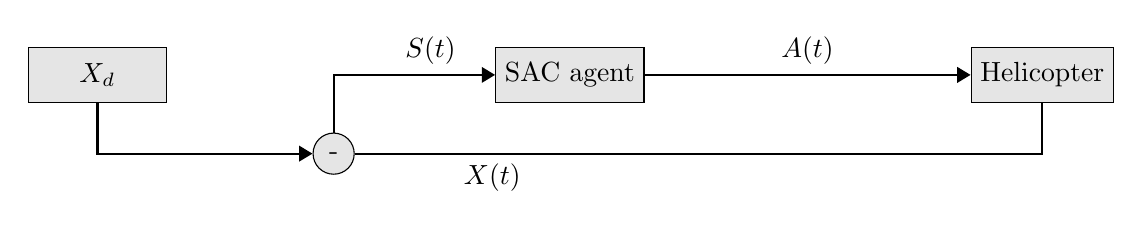
\begin{tikzpicture}[auto,node distance=2cm,scale=1.0]
		\node [block,fill=gray!20,](Xd){$X_d$};
		\node [input, right of=Xd, node distance=3cm](sum1){};
		\node [block, fill=gray!20, right of=sum1, node distance=3cm](SAC){SAC agent};
		\node [block, fill=gray!20, right of=SAC, node distance=6cm](plant){Helicopter};
		\node [sum, fill=gray!20, below of=sum1, distance=7m](ypos){-};
		\node [input, below of=sum1](belowsum){};
		\node [input, right of=sum1,node distance=1cm](rightsum){};
		\node [output, right of=plant](out1){};
		\node [output, below of=out1](out2){};
		\draw [arrow] (SAC)--node{$A(t)$}(plant);
		\draw [line] (plant)|- node [pos=0.90]{$X(t)$} (ypos);
		\draw [arrow] (Xd)|-(ypos);
		\draw [arrow] (ypos)|-node[pos=0.80]{$S(t)$}(SAC);
	\end{tikzpicture}
	\caption{SAC controller schematic}
	\label{SAC_controller}
\end{figure}

\subsection{Architecture}

In this section, we discuss the architecture of the SAC actor and critic neural network.

\subsubsection*{Actor}

The actor diagram and schematic of this SAC agent is given in figures \cref{actor_diagram,nnschematic} which includes 2 hidden layer of size 128 and 128 fully connected layers with a Rectified Linear Unity (RelU) activation function and a $tanh$ activation function at last in order to narrow the result to [-1,1], the actions are then linearly mapped to the action range based on the environment\footnote{check action wrapper at Appendix A}. In order to constraint the standard deviation of the policy, it is set to be between $[e^{-20},e^{1}]$.

\begin{figure} 
	\centering
	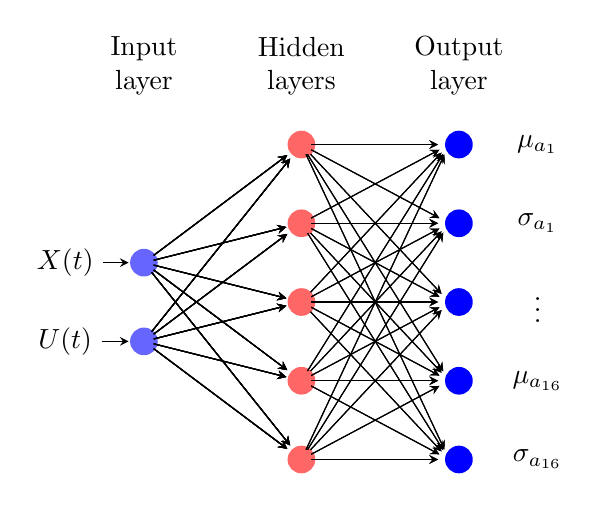
\begin{tikzpicture}[every node/.style={align=center}]
		\foreach \x in{1,2,3,4,5}
		\fill[red!60](0,\x)circle(5pt)node(a\x){};
		
		\fill[blue!60](-2,2.5)circle(5pt)node(b3){};
		\fill[blue!60](-2,3.5)circle(5pt)node(b4){};
		\fill[blue](2,2)circle(5pt)node(c1){};
		\fill[blue](2,3)circle(5pt)node(c2){};
		\fill[blue](2,4)circle(5pt)node(c3){};
		\fill[blue](2,5)circle(5pt)node(c4){};
		\fill[blue](2,1)circle(5pt)node(c5){};
		\node(y4)at(-3,3.5){$X(t)$};
		\node(y3)at(-3,2.5){$U(t)$};
		
		
		\node at(-2,6){Input\\layer};
		\node at(0,6){Hidden\\layers};
		\node at(2,6){Output\\layer};
		\node(d4)at(3,5){$\mu_{a_1}$};
		\node(d3)at(3,4){$\sigma_{a_1}$};
		\node(d2)at(3,3){$\vdots $};
		\node(d1)at(3,2){$\mu_{a_{16}}$};
		\node(d5)at(3,1){$\sigma_{a_{16}}$};
		\foreach \x in{3,4}
		\draw[-{stealth[sep=2pt]}](y\x)--(b\x);
		\foreach \x in{3,4}
		{\foreach \y in{1,2,3,4,5}
			\foreach \z in {1,2,3,4,5}
			{
				{\draw[-{stealth[sep=2pt]}](b\x)--(a\y);
					\draw[-{stealth[sep=4pt]}](a\y)--(c\z.west);
				}
			}
			c}
	\end{tikzpicture}
	\caption{Actor diagram for SAC agent, the inputs are the 16 states of the helicopter $X(t)$ and the 4 control inputs $U(t)$, the outputs are the average $\mu$ and the standard deviation $\sigma$ of the agent actions}
	\label{actor_diagram}
\end{figure}

\subsubsection*{Critic}

The diagram for the Critic neural network is depicted in \cref{critic_diagram,nnschematic}.
The diagram includes 2 hidden layer of size 256 and 256 fully connected layers with RelU activation function after each hidden layers.

\begin{figure} 
	\centering
	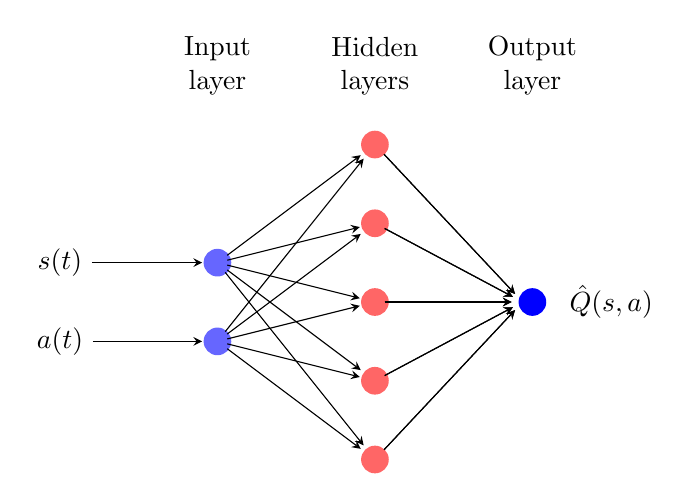
\begin{tikzpicture}[every node/.style={align=center}]
		\foreach \x in{1,2,3,4,5}
		\fill[red!60](0,\x)circle(5pt)node(a\x){};
		\fill[blue!60](-2,2.5)circle(5pt)node(b1){};
		\fill[blue!60](-2,3.5)circle(5pt)node(b2){};
		\fill[blue](2,3)circle(5pt)node(c1){};
		\node(y2)at(-4,3.5){$s(t)$};
		\node(y1)at(-4,2.5){$a(t)$};
		\node at(-2,6){Input\\layer};
		\node at(0,6){Hidden\\layers};
		\node at(2,6){Output\\layer};
		
		\node(d1)at(3,3){$\hat{Q}(s,a)$};
		
		\foreach \x in{1,2}
		\draw[-{stealth[sep=2pt]}](y\x)--(b\x);
		\foreach \x in{1,2}
		{\foreach \y in{1,2,3,4,5}
			\foreach \z in {1}
			{
				{\draw[-{stealth[sep=2pt]}](b\x)--(a\y);
					\draw[-{stealth[sep=4pt]}](a\y)--(c\z.west);
				}
			}
			c}
	\end{tikzpicture}
	\caption{Critic diagram for SAC agent, inputs are the states and actions while the output is the Q value for the given input.}
	\label{critic_diagram}
\end{figure}

\begin{figure} 
	\centering
	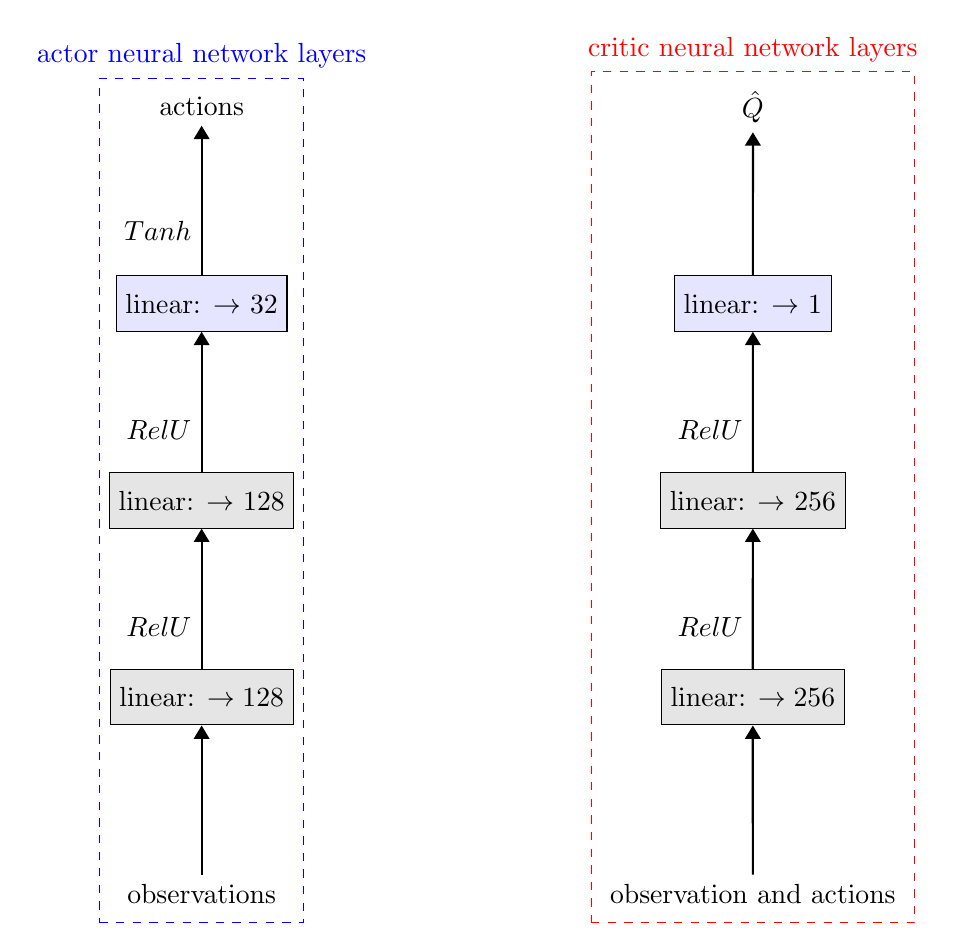
\begin{tikzpicture}[auto,node distance=2.5cm,scale=0.4]
		\node [block,fill=gray!20,](firstlayer){linear: $\rightarrow 128$};
		\node [below of=firstlayer](input){observations};
		\node [block, fill=gray!20, above of=firstlayer, node distance=2.5cm](secondlayer){linear: $\rightarrow$ 128};
		\node [block, above of=secondlayer, node distance=2.5cm](thirdlayer){linear: $\rightarrow$ 32};
		\node [above of=thirdlayer, node distance=2.5cm](actions){actions};
		
		
		\node [block, right of= firstlayer,fill=gray!20,node distance=7cm](flayercritic){linear: $\rightarrow 256$};
		\node [below of=flayercritic](criticinput){observation and actions};
		\node [block, fill=gray!20, above of=flayercritic, node distance=2.5cm](slayercritic){linear: $\rightarrow$ 256};
		\node [block, above of=slayercritic, node distance=2.5cm](thlayercritic){linear: $\rightarrow$ 1};
		\node [above of=thlayercritic, node distance=2.5cm](atoms){$\hat{Q}$};
		
		\draw [arrow] (input)--(firstlayer);
		\draw [arrow] (firstlayer)--node[pos=0.30]{$RelU$}(secondlayer);
		\draw [arrow] (secondlayer) --node[pos=0.30]{$RelU$}(thirdlayer);
		\draw [arrow] (thirdlayer) --node[pos=0.30]{$Tanh$}(actions);
		
		\draw [arrow] (criticinput)--(flayercritic);
		
		
		\draw [arrow] (flayercritic)--node[pos=0.30]{$RelU$}(slayercritic);
		\draw [arrow] (slayercritic) --node[pos=0.30]{$RelU$}(thlayercritic);
		\draw [arrow] (thlayercritic) --node[pos=0.20]{}(atoms);
		\node[fit=(firstlayer)(input)(secondlayer)(thirdlayer)(actions),draw,blue,dashed,
		label={[blue]above: actor neural network layers}]{};
		\node[fit=(flayercritic)(criticinput)(slayercritic)(thlayercritic)(atoms),draw,red,dashed,label={[red]above: critic neural network layers}]{};
	\end{tikzpicture}
	\caption{Actor and critic neural network diagram}
	\label{nnschematic}
\end{figure}

\subsection{Hyper-parameters}

Optuna package is utilized for optimization of all the hyperparameters of the SAC agent \cite{optuna_2019}. The SAC agent's primary hyper-parameters are given in table \ref{table of hyperparameters} as part of its implementation.
\begin{longtable}{c|c|c} 
	\caption {Hyper parameters of SAC agent.}\label{table of hyperparameters}\\\toprule
	\endfirsthead
	\caption* {\textbf{Table \ref{table of hyperparameters} Continued:} }\\\toprule
	\endhead
	\endfoot
	\bottomrule
	\endlastfoot
		\textbf{Hyper parameter} & \textbf{Value} & \textbf{description}  \\ \hline \hline
$\mathcal{T}$ & $5\times10^{7}$ &  Total number of environment steps.\\&& \\ \hline
$\mathcal{B}$ & 2048  & mini batch which is the number of samples\\&& from the buffer randomly sampled for each\\&& stochastic gradient decent step update\\&& \\ \hline
$\mathcal{D}$ & $10^7$  &replay buffer size, which is the total number\\&& of steps saved in buffer (when new ones are\\&& added the oldest ones are removed.)\\&& \\ \hline
$\l_{\kappa}$  & $3\times 10^{-4}$  & learning rate for optimization of policy \\&& by this factor.\\&& \\ \hline
$\l_{\delta}$  & $3\times 10^{-4}$  & learning rate for optimization of Q functions.\\&& \\ \hline
$\tau_{target}$  & $5\times 10^{-3}$  & updating the target network linearly\\&& by this factor.\\&& \\ \hline
$\gamma$  & 0.99  &  factor for discounting later rewards.\\&& \\ \hline
$\alpha$  & $3\times e^{-0.009i}$ & the temperature term in SAC policy.\\&& \\ \hline
$\chi$  & $3\times 10^{-3}$  & The learning rate of Adam optimizer.\\&& \\ \hline
$\sigma_{mean}$  & $e^{-20}$  & the minimum standard deviation of the\\&& actions in the stochastic policy of SAC.\\&& \\ \hline
$\sigma_{mean}$  & $e^{1}$  &  the maximum standard deviation of the\\&& actions in the stochastic policy of SAC\\&& \\ \hline
$i_{max}$  & $10^4$  &  the maximum  number of iteration\\&& \\ \hline
\end{longtable}

The replay buffer is designed to contain $10^7$ transition tuples before starting the SAC algorithm. The experience replay buffer enables learning from prior policy experiences while avoiding correlated samples in the gradient step. Furthermore, we implement an upgraded target network with a target factor of $5\times10^{-3}$.This is motivated by the desire to improve the stability of the learning process. Based on line 21 of algorithm \ref{sac algorithm}, if it is time to update, the gradient step  per epoch is set to 2 and the gradient step per iteration is set to 8. For each time a gradient step is executed, a mini-batch of 2048 random samples is chosen from the replay buffer. The learning rate for Adam optimizer on both neural network is set to be $3\times10^{-3}$.

The training of the network included about $5\times10^{7}$ to  $6\times10^{7}$ environment time steps of about 0.03, simulation time. The simulation is run in a 32-cores Intel(R) Xeon(R) CPU E5-2620 v4 @ 2.10GHz which took about 3–4 days.

\section{Results}

\subsection{Training and evaluation}

The training result is given in \ref{ave_return}. The iteration is continued for 10,000 iterations; however, no significant improvement is found after 6000. The standard deviation increases as the number of iterations increases. This is acceptable because at first, in all the episodes, the simulated UAV crashes. However, as the training progresses, the agent improves its action to stabilize the helicopter and hence the difference between the return of points closer to the origin and those placed at a more distant point from the origin grows.

\begin{figure}
	\begin{center}
		\hbox{\hspace*{-2.5cm} 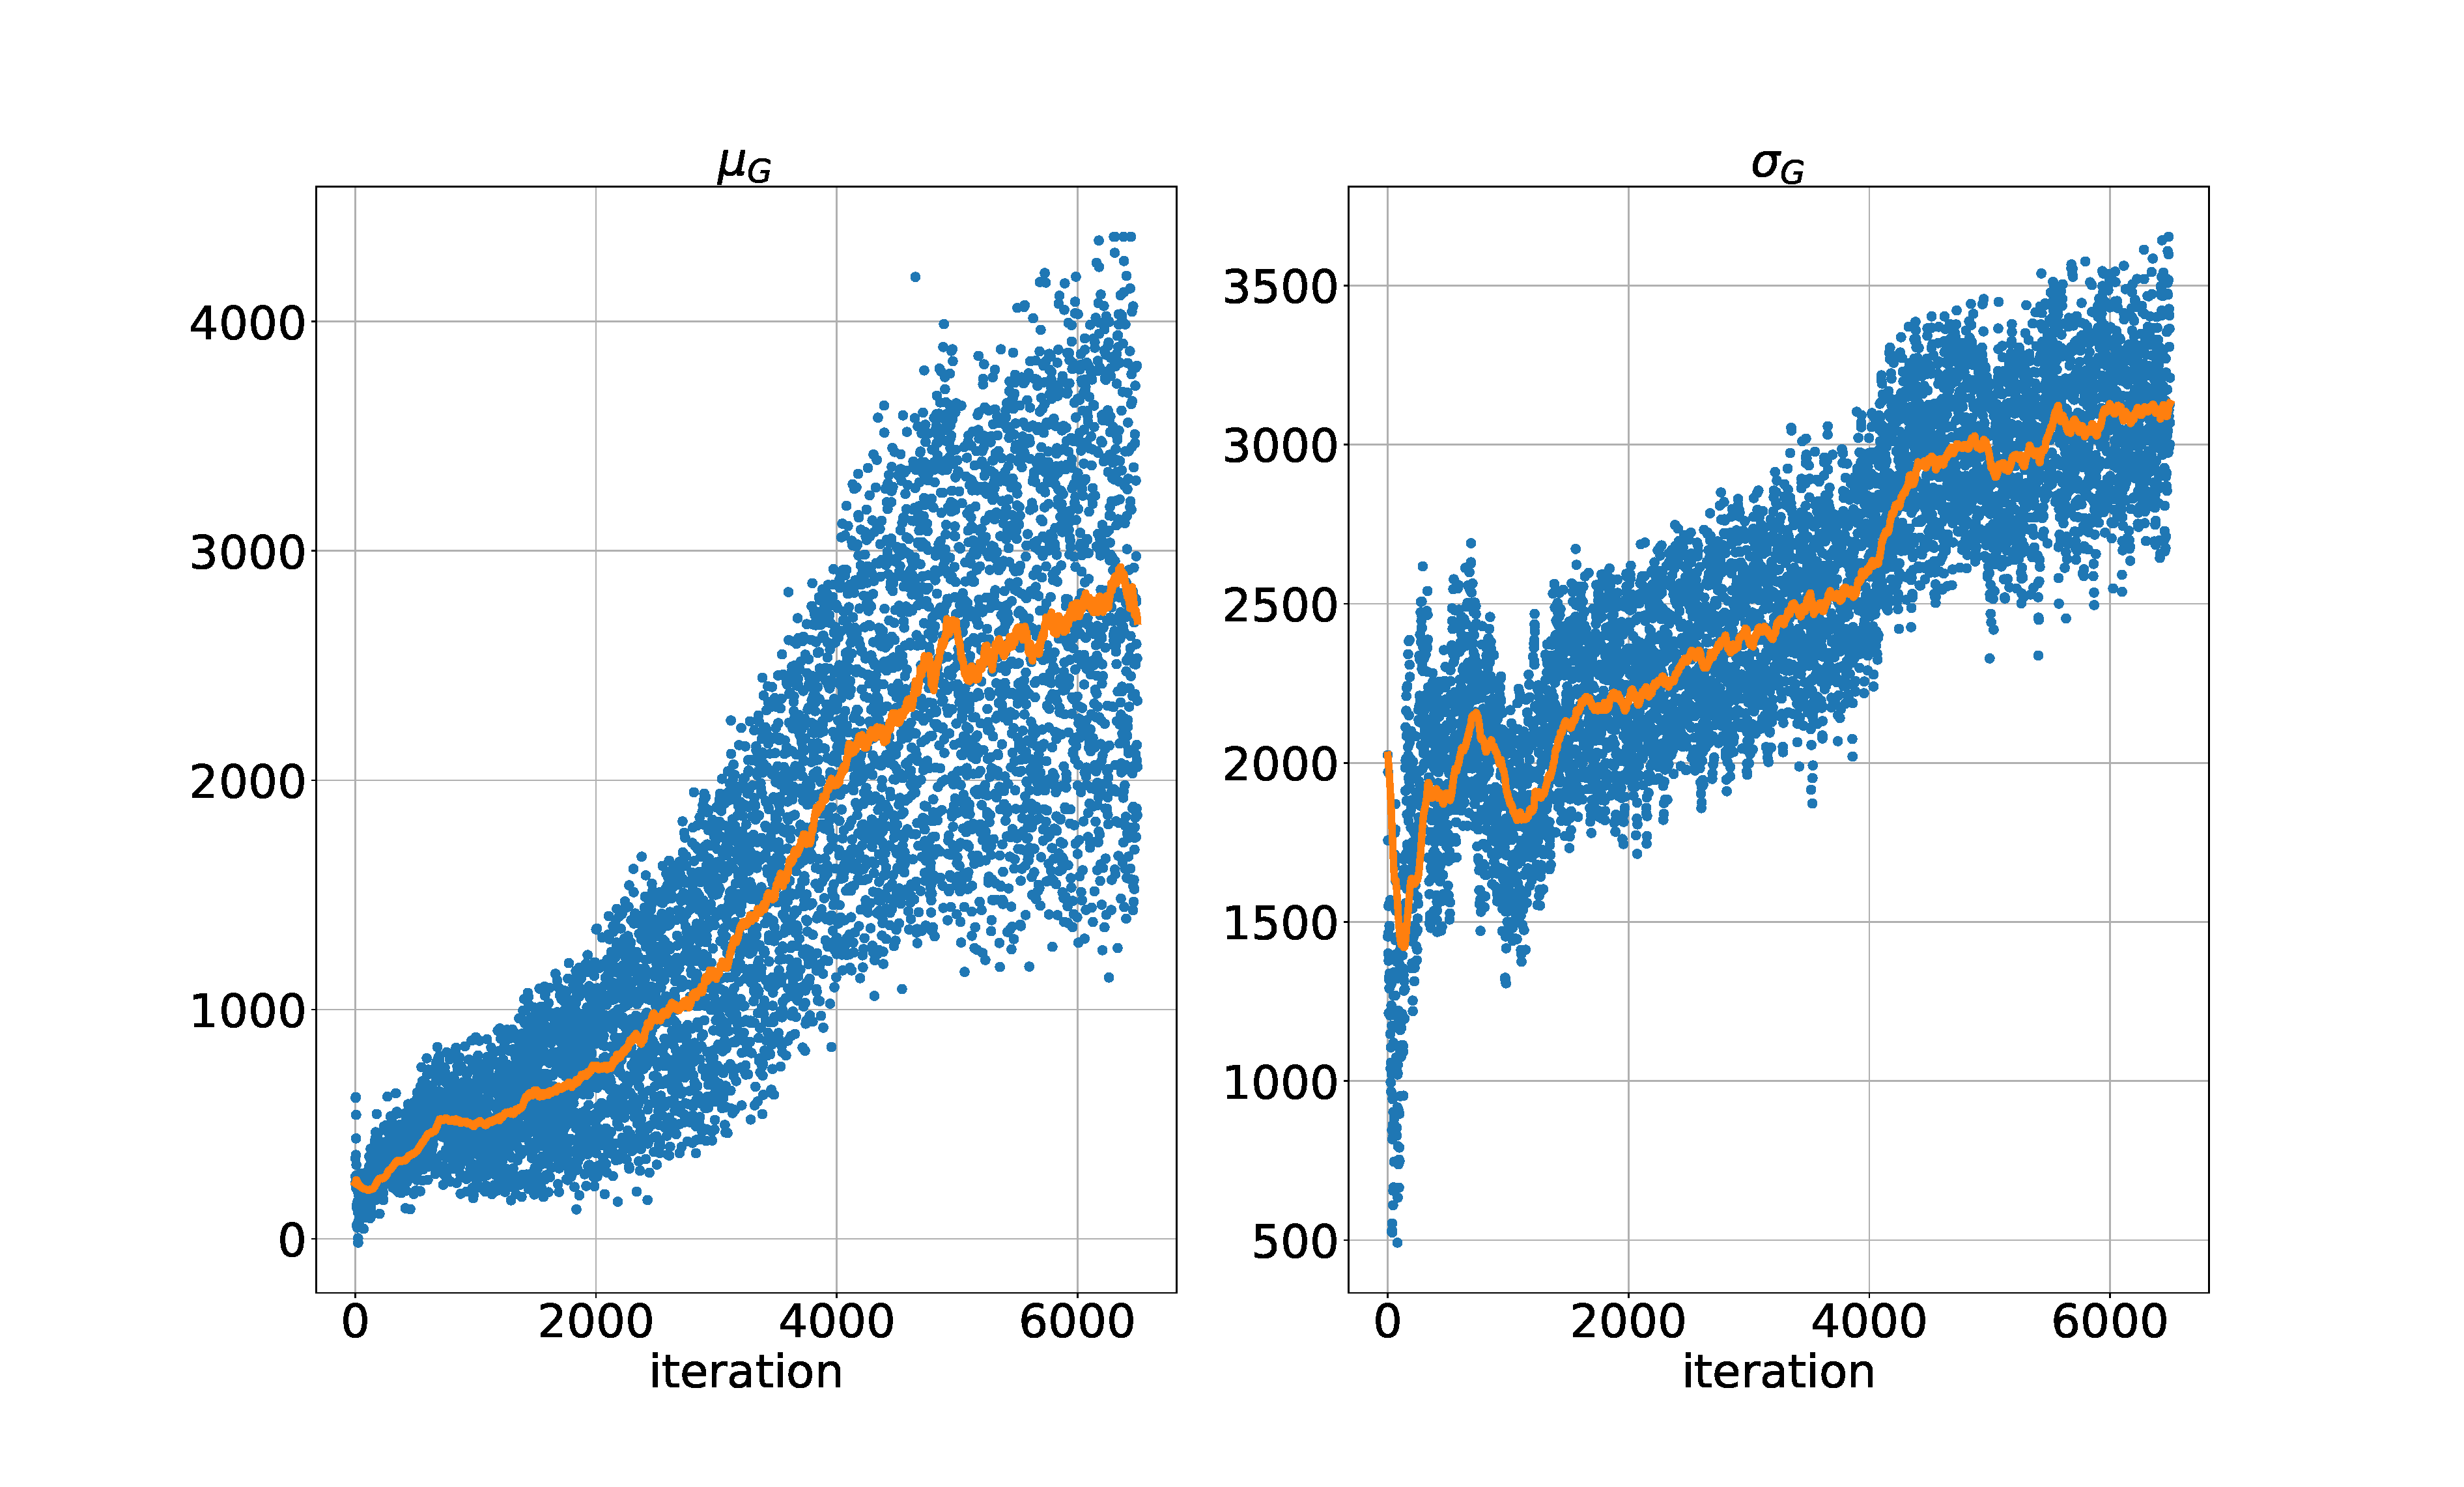
\includegraphics[scale=0.31]{avereturn.eps}}

		\caption{Averaged discounted return $\mu_G$ and standard deviation $\sigma_G$ of each iteration using the random actions of the policy.}
		\label{ave_return}
	\end{center}
\end{figure}

\subsection{Comparison of Controllability and stability to the SMC}

In order to be able to compare the results obtained by an RL method to a traditional control method, the results of controlling the initial point set to [-1,-1,-1] are shown in \cref{states,omega,theta,v_res,actions_delta,flapping} for both the sliding mode controller (SMC) and the SAC policy obtained. As seen, the resulting policy achieves good stabilization capability.

The settling time is considered to be the time when the states reach 0.10 m of the origin which is the desired state. The rise time in this study is considered to be the time for the response to rise from the absolute value of 0.9 m to 0.1 m in the vicinity of origin for each x, y and z states. Considering the aforementioned definitions the comparison between the SAC and SMC is given in table \ref{SAC_SMC}.

\begin{longtable}{c||c|c|c|c} 
	\caption {Comparison of SAC and SMC based on the response characteristics of the helicopter dynamic system for the case of initial point set to [-1,-1,-1].}\label{SAC_SMC}\\\toprule
	\endfirsthead
	\caption* {\textbf{Table \ref{SAC_SMC} Continued:} }\\\toprule
	\endhead
	\endfoot
	\bottomrule
	\endlastfoot
	\textbf{} & \textbf{settling time [s]} & \textbf{rise time [s]} & \textbf{overshoot [m]} & \textbf{SS error [m]}  \\ \hline \hline
	\textbf{x,SMC} & 5.07 & \textbf{0.79} & 0.13 & 0.0  \\ 
	\textbf{x,SAC} & \textbf{4.41} & 3.96 & \textbf{0} & 0  \\ \hline
	
	\textbf{y,SMC} & \textbf{1.36} & \textbf{1.0} & 0.09 & 0.05  \\ 
	\textbf{y,SAC} & 2.96 & 2.66 & \textbf{0} & 0.05  \\ \hline
	
	\textbf{z,SMC} & \textbf{1.51} & \textbf{1.47} & \textbf{0.03} & \textbf{0}  \\ 
	\textbf{z,SAC} & 2.6 & 2.45 & 0.1 & 0.1  \\
	
\end{longtable}

Based on the given comparison result on \ref{SAC_SMC} the sliding mode controller provides a better result in the case of x y and z. The $\psi$ angle has a $10.8^{\circ}$ steady-state error which is not superior to the sliding mode controller ($1.8^{\circ}$). However, it should be mentioned that the sliding mode controller is a highly tuned controller for this system. On the other hand, the SAC agent is a model-free method in which it did not have any access to the model. 

The result of the control input is given in figure \ref{actions_delta}. There are some vibrations in the $\delta_{ped}$ and $\delta_{col}$, We find that it was somewhat hard to reduce these vibrations because as we increased the control derivative input term in the \ref{control_reward}, the policy would alternate between getting closer to the target and achieving a stable hovering somewhere far from the origin. 

\subsubsection {robustness}

In order to test the robustness of the policy, a simulated wind is blown at the UAV given the following equation:

\begin{equation}
	V_{wind,t}=V_{wind,t-1}+ W
\end{equation}

in which W is a random number in [-0.1,0.1] at each time step and using the policy generated. It achieved 100\% stability in all the 27 initial positions, In order to compare the results of the simulation with and without the wind, the rise time, settling time, and steady-state errors are given in table \ref{wind_sac} for the [-1,-1,-1] case.

\begin{longtable}{c||c|c|c|c} 
	\caption {Robustness response characteristics of the helicopter dynamic system  for the SAC policy by a simulated wind for the case of initial point set to [-1,-1,-1].}\label{wind_sac}\\\toprule
	\endfirsthead
	\caption* {\textbf{Table \ref{wind_sac} Continued:} }\\\toprule
	\endhead
	\endfoot
	\bottomrule
	\endlastfoot
	\textbf{} & \textbf{settling time [s]} & \textbf{rise time [s]} & \textbf{overshoot [m]} & \textbf{SS error [m]}  \\ \hline \hline
	\textbf{x} & 4.29 & 3.87 & 0 & 0.03  \\ \hline
	\textbf{y} & 2.87 & 2.57 & 0.08 & 0.02  \\ \hline
	\textbf{z} & 2.47 & 2.36 & 0.09 & 0.09  \\
	
\end{longtable}

\begin{figure}
	\begin{center}
		{\includegraphics[scale=0.41]{X.pdf}}
		\caption{Helicopter SMC and SAC positional states by initial position [-1,-1,-1].}
		\label{states}
	\end{center}
\end{figure}

\begin{figure}
	\begin{center}
		{\includegraphics[scale=0.41]{omega.pdf}}
		\caption{Helicopter SMC and SAC angular velocities by initial position [-1,-1,-1].}
		\label{omega}
	\end{center}
\end{figure}

\begin{figure}
	\begin{center}
		{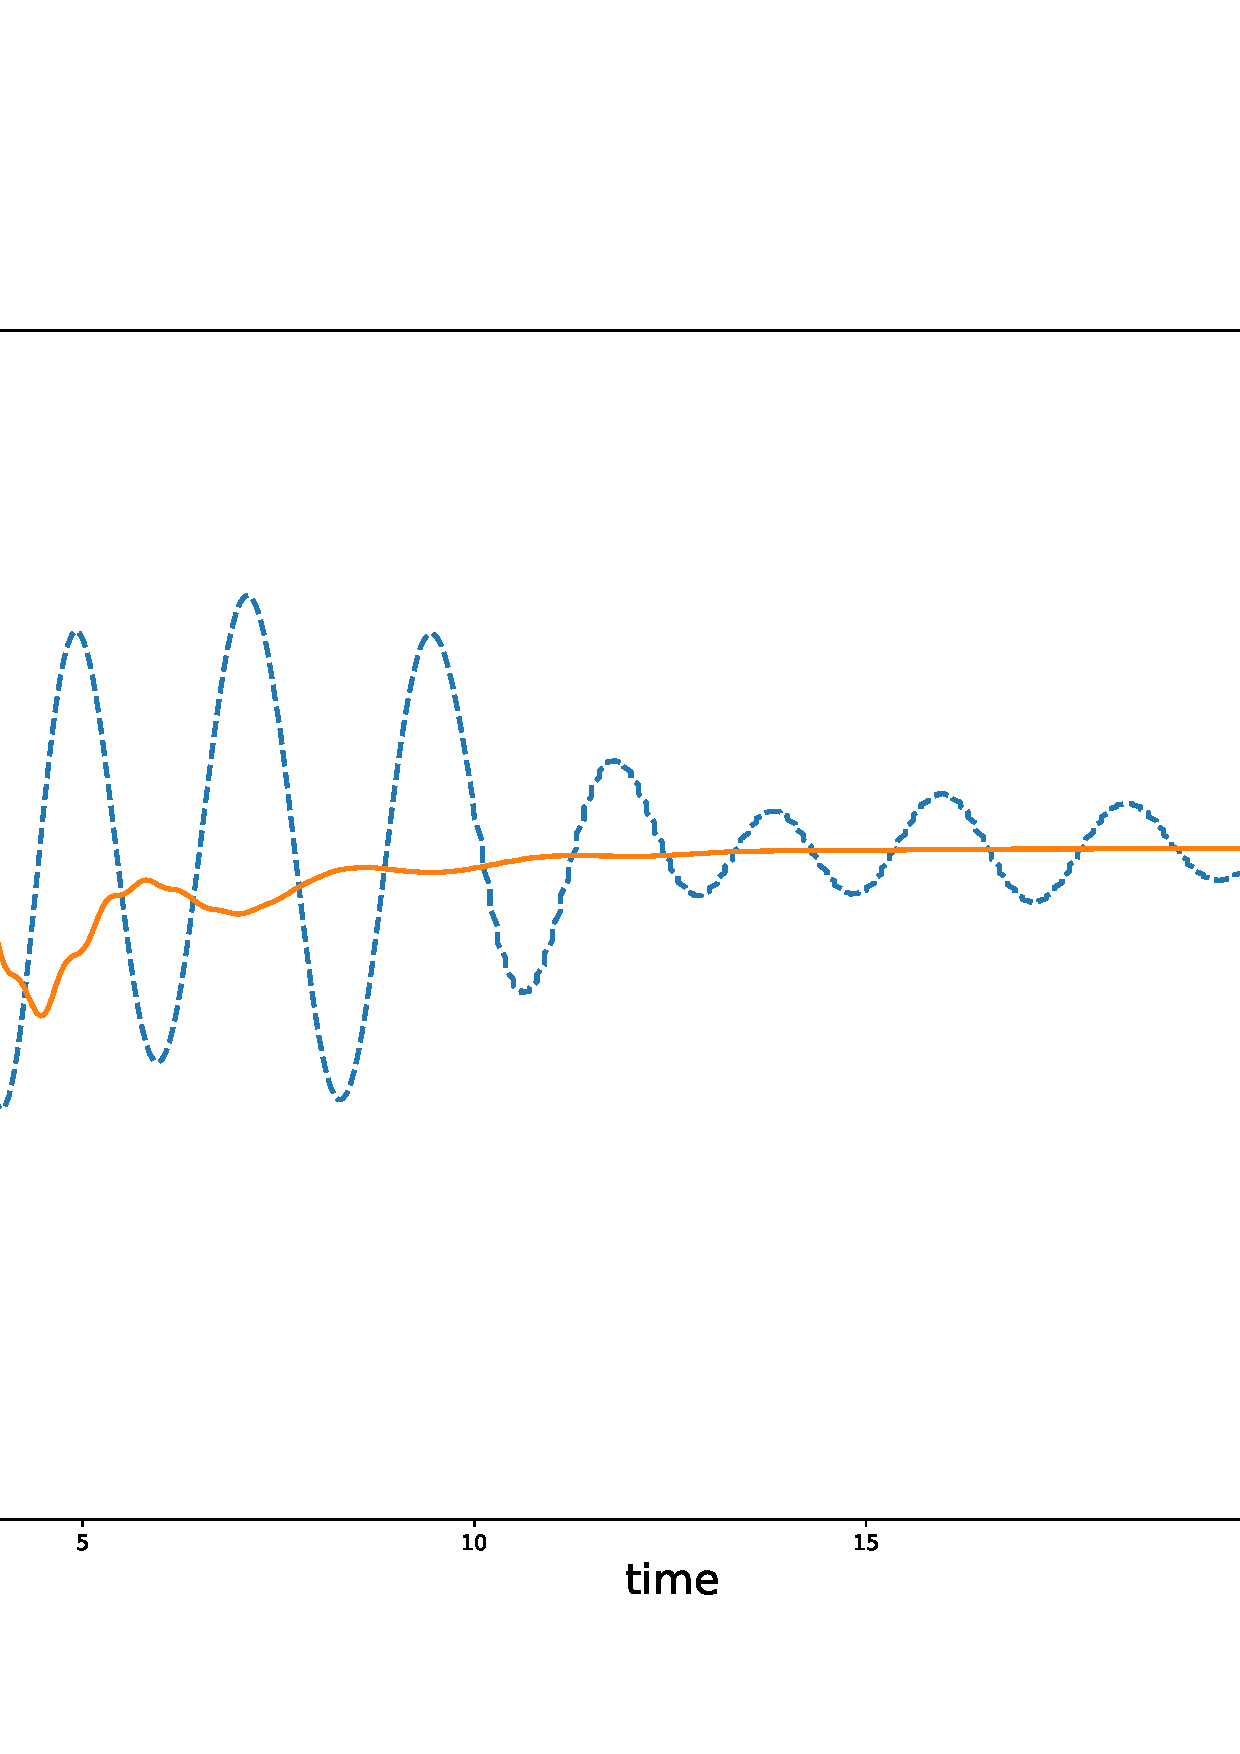
\includegraphics[scale=0.41]{theta.pdf}}
		\caption{Helicopter SMC and SAC Euler angles by initial position [-1,-1,-1].}
		\label{theta}
	\end{center}
\end{figure}

\begin{figure}
	\begin{center}
		{\includegraphics[scale=0.41]{V.pdf}}
		\caption{Helicopter SMC and SAC velocities by initial position [-1,-1,-1].}
		\label{v_res}
	\end{center}
\end{figure}

\begin{figure}
	\begin{center}
		{\includegraphics[scale=0.41]{col.pdf}}
		\caption{Helicopter SMC and SAC control input by initial position [-1,-1,-1].}
		\label{actions_delta}
	\end{center}
\end{figure}

\begin{figure}
	\begin{center}
		{\includegraphics[scale=0.41]{flapping.pdf}}
		\caption{Helicopter SMC and SAC flapping states by initial position [-1,-1,-1].}
		\label{flapping}
	\end{center}
\end{figure}
\chapter{Conclusions and Future Directions}

\section{Conclusions}

This study shows how to train a reinforcement learning agent using a model-free off-policy technique, specifically the Soft Actor-Critic algorithm, to produce a policy capable of performing low-level control of a simulated small-scaled helicopter. The use of this method for the same task has never been disclosed previously. The result of the SAC method is compared to an sliding mode controller, although the result was not superior, having in mind that the SAC method did not have access to the dynamics of the simulated helicopter, it provided a promising result in which the average steady state error was 0.05\% for the given [-1,-1,-1] case while the sliding mode controller provided an almost 0 error on the steady states. We also assessed the policy in an environment with the random wind as a disturbance to test the robustness of the method, and it is demonstrated that the SAC technique was capable of achieving stability in all trials. 

\section{Future work}
The comparison of the results in the previous section showed that there is still room for improvement in case if stability criteria of the achieved policy, one way to improve it is to work in more detail about the reward function of the policy, another procedure would be to improve the RL algorithms by modifications as the RL field is improving day by day. 
Although it was demonstrated here that the small-sized helicopter could be stabilized using the SAC approach, trajectory tracking and recovery operations were not conducted in this study and can be addressed in future studies. In \cite{barros2020using}, similar study was conducted on a quadcopter.

The ability to efficiently apply deep RL algorithms to the real world to address practical applications may be the most compelling motivator for future advances in the area.
This study showed that RL is capable of controlling the helicopter; however, this has been done in the simulation environment, future studies could be focused on using such policies in real-world data. A review of similar approaches may be found in \cite{zhao2020sim}.

There is a possibility of a relatively large gap between the simulation environment and the real-world data; a possible moderator would be to take advantage of a more sophisticated model such as the one for Yamaha R-50 helicopter \cite{la2003integrated,civita2006design} to improve the replication of the environment.







%% This defines the bibliography file (main.bib) and the bibliography style.
%% If you want to create a bibliography file by hand, change the contents of
%% this file to a `thebibliography' environment.  For more information
%% see section 4.3 of the LaTeX manual.
\begin{singlespace}
\clearpage\addcontentsline{toc}{chapter}{Bibliography}
%\bibliographystyle{IFAC}
\bibliographystyle{unsrt}
\bibliography{refs}
\end{singlespace}




\appendix
\renewcommand\thefigure{\Alph{section}S.\arabic{figure}}


\appendix

\section*{Appendix A} \label{appendix1}
The code of the helicopter environment. The full library is available at \href{https://github.com/MKamyab1991/sac_helicopter.git}{github}.

\lstset{caption={Helicopter environment algorithm.}}
\lstinputlisting[language=Python]{helicopter_env.py}


%\section*{Approximation of the extension ratio}

\include{appb}

%\singlespacing
%\bibliographystyle{plain}
%\bibliography{biblio}
\end{document}

